\documentclass[12pt]{article}
\usepackage{fontspec}
\usepackage{fullpage}
\usepackage{hyperref}
\hypersetup{bookmarks=true,colorlinks=true,linkcolor=red,citecolor=blue,filecolor=magenta,urlcolor=cyan}
\usepackage{amsmath}
\usepackage{amssymb}
\usepackage{mathtools}
\usepackage{unicode-math}
\usepackage{tabu}
\usepackage{longtable}
\usepackage{booktabs}
\usepackage{caption}
\usepackage{graphics}
\usepackage{enumitem}
\usepackage{filecontents}
\usepackage[backend=bibtex]{biblatex}
\usepackage{url}
\newlist{symbDescription}{description}{1}
\setlist[symbDescription]{noitemsep, topsep=0pt, parsep=0pt, partopsep=0pt}
\setmathfont{Latin Modern Math}
\global\tabulinesep=1mm
\bibliography{bibfile}
\title{Software Requirements Specification for Slope Stability analysis Program}
\author{Henry Frankis}
\begin{document}
\maketitle
\tableofcontents
\newpage
\section{Reference Material}
\label{Sec:RefMat}
This section records information for easy reference.
\subsection{Table of Units}
\label{Sec:ToU}
The unit system used throughout is SI (Système International d'Unités). In addition to the basic units, several derived units are also used. For each unit, the table lists the symbol, a description and the SI name.
\begin{longtable*}{l l}
\toprule
Symbol & Description
\\
\midrule
\endhead
${}^{\circ}$ & angle (degree)
\\
m & length (metre)
\\
N & force (newton)
\\
Pa & pressure (pascal)
\\
\bottomrule
\label{Table:ToU}
\end{longtable*}
\subsection{Table of Symbols}
\label{Sec:ToS}
The table that follows summarizes the symbols used in this document along with their units. Throughout the document, values with a subscript $i$ implies that the value will be taken at and analyzed at a slice or slice interface composing the total slip mass.
\begin{longtabu}{l X[l] l}
\toprule
Symbol & Description & Units
\\
\midrule
\endhead
$(x,y)$ & Cartesian Position Coordinates: y is considered parallel to the direction of the force of gravity and x is considered perpendicular to y & m
\\
$A$ & Area: A part of an object or surface & $\text{m}^{2}$
\\
$b$ & Base Width of a Slice: in the x-direction & m
\\
${C_{den}}$ & Proportionality Constant Denominator: expression used to calculate the denominator of the interslice normal to shear force proportionality constant & N
\\
${C_{num}}$ & Proportionality Constant Numerator: expression used to calculate the numerator of the interslice normal to shear force proportionality constant & N
\\
$c'$ & Effective Cohesion: internal pressure that sticks particles of soil together & Pa
\\
$const_f$ & Decision on F: boolean decision on which form of f the user desires: constant if true, or half-sine if false & --
\\
$f$ & Interslice Normal to Shear Force Ratio Variation Function: function of distance in the x-direction & --
\\
${F_{S}}$ & Factor of Safety: The global stability metric of a slip surface of a slope, defined as the ratio of resistive shear force to mobilized shear force & --
\\
${F_{x}}$ & X-Component of the Net Force:  & N
\\
${F_{y}}$ & Y-Component of the Net Force:  & N
\\
${{F_{S}}^{min}}$ & Minimum Factor of Safety: The minimum factor of safety associated with the critical slip surface & --
\\
${{F_{x}}^{G}}$ & Sum of the Interslice Normal Forces: for two adjacent interslice boundaries & N
\\
${{F_{x}}^{H}}$ & Sum of the Interslice Normal Water Forces: for two adjacent interslice boundaries & N
\\
$\mathbf{F}$ & Force: An interaction that tends to produce change in the motion of an object & N
\\
$G$ & Interslice Normal Force: per meter in the z-direction exerted between adjacent slices & $\frac{\text{N}}{\text{m}}$
\\
$H$ & Interslice Normal Water Force: per meter in the z-direction exerted in the x-ordinate direction between adjacent slices & $\frac{\text{N}}{\text{m}}$
\\
$h$ & Y-Direction Height of a Slice: height in the y-direction from the base of a slice to the slope surface, at the x-direction midpoint of the slice & m
\\
${h^{L}}$ & Height of the Left Side of a Slice: assuming slice surface has negative slope & m
\\
${h^{R}}$ & Height of the Right Side of a Slice: assuming slice surface has negative slope & m
\\
${h_{z}}$ & Height of Center of Slice: the height in the y-direction from the base of a slice to the center of the slice & m
\\
${h_{z,w}}$ & Height Halfway to Water Table: the height in the y-direction from the base of a slice halfway to the water table & m
\\
$i$ & Index: representing a single slice & --
\\
${K_{c}}$ & Seismic Coefficient: proportionality factor of force that weight pushes outwards; caused by seismic earth movements & --
\\
$M$ & Net Moment: a measure of the tendency of a body to rotate about a specific point or axis & Nm
\\
$N$ & Normal Force: total reactive force per meter in the z-direction for a soil surface subject to a body resting on it & $\frac{\text{N}}{\text{m}}$
\\
$n$ & Number of Slices: the slip mass has been divided into & --
\\
$N'$ & Effective Normal Force: per meter in the z-direction for a soil surface, subtracting pore water reactive force from total reactive force & $\frac{\text{N}}{\text{m}}$
\\
$P$ & Resistive Shear Force: Mohr Coulomb frictional force per meter in the z-direction that describes the limit of mobilized shear force a slice can withstand before failure & $\frac{\text{N}}{\text{m}}$
\\
$Q$ & External Force: a force per meter in the z-direction acting into the surface from the midpoint of a slice & $\frac{\text{N}}{\text{m}}$
\\
$R$ & Resistive Shear Force Without the Influence of Interslice Forces: per meter in the z-direction & $\frac{\text{N}}{\text{m}}$
\\
$S$ & Mobilized Shear Force: per meter in the z-direction & $\frac{\text{N}}{\text{m}}$
\\
$T$ & Mobilized Shear Force Without the Influence of Interslice Forces: per meter in the z-direction & $\frac{\text{N}}{\text{m}}$
\\
$u$ & Pore Pressure: from water within the soil & Pa
\\
${U_{b}}$ & Base Hydrostatic Force: per meter in the z-direction from water pressure within a slice & $\frac{\text{N}}{\text{m}}$
\\
${U_{t}}$ & Surface Hydrostatic Force: per meter in the z-direction from water pressure acting into the slice from standing water on the slope surface & $\frac{\text{N}}{\text{m}}$
\\
${{U^{L}}_{b}}$ & Left Base Hydrostatic Force on a Slice: per meter in the z-direction from water pressure within a slice, assuming the entire slice has the height of the left side of the slice & $\frac{\text{N}}{\text{m}}$
\\
${{U^{L}}_{t}}$ & Left Surface Hydrostatic Force on a Slice: per meter in the z-direction from water pressure acting into the slice from standing water on the slope surface, assuming the entire slice has the height of the left side of the slice & $\frac{\text{N}}{\text{m}}$
\\
${{U^{R}}_{b}}$ & Right Base Hydrostatic Force on a Slice: per meter in the z-direction from water pressure within a slice, assuming the entire slice has the height of the right side of the slice & $\frac{\text{N}}{\text{m}}$
\\
${{U^{R}}_{t}}$ & Right Surface Hydrostatic Force on a Slice: per meter in the z-direction from water pressure acting into the slice from standing water on the slope surface, assuming the entire slice has the height of the right side of the slice & $\frac{\text{N}}{\text{m}}$
\\
$v$ & Local Index: used as a bound variable index in calculations & --
\\
$W$ & Weight: downward force per meter in the z-direction caused by gravity on slice i & $\frac{\text{N}}{\text{m}}$
\\
${W^{L}}$ & Left Weight of a Slice: weight of a slice per meter in the z-direction, assuming the entire slice has the height of the left side of the slice & $\frac{\text{N}}{\text{m}}$
\\
${W^{R}}$ & Right Weight of a Slice: weight of a slice per meter in the z-direction, assuming the entire slice has the height of the right side of the slice & $\frac{\text{N}}{\text{m}}$
\\
$X$ & Interslice Shear Force: per meter in the z-direction exerted between adjacent slices & $\frac{\text{N}}{\text{m}}$
\\
${x_{slip}}$ & X-Coordinate of the Slip Surface: distance of the slip surface & m
\\
${x_{slope}}$ & X-Coordinate of the Slope: x-coordinate of a point on the slope & m
\\
${x_{wt}}$ & X-Coordinate: x-position of the water table & m
\\
${y_{slip}}$ & Y-Coordinate of the Slip Surface: height of the slip surface & m
\\
${y_{slope}}$ & Y-Coordinate of the Slope: y-coordinate of a point on the soil slope & m
\\
${y_{wt}}$ & Y-Coordinate of the Water Table: height of the water table & m
\\
$z$ & Z-Coordinate: in the Cartesian coordinate system & m
\\
$α$ & Base Angle: between the base of a slice and the horizontal & ${}^{\circ}$
\\
$β$ & Surface Angle: between the surface of a slice and the horizontal & ${}^{\circ}$
\\
$γ$ & Soil Dry Unit Weight: The weight of a dry soil/ground layer divided by the volume of the layer. & $\frac{\text{N}}{\text{m}^{3}}$
\\
${γ_{Sat}}$ & Soil Saturated Unit Weight: The weight of saturated soil/ground layer divided by the volume of the layer. & $\frac{\text{N}}{\text{m}^{3}}$
\\
${γ_{w}}$ & Unit Weight of Water: The weight of one cubic meter of water. & $\frac{\text{N}}{\text{m}^{3}}$
\\
$λ$ & Proportionality Constant: for the interslice normal to shear force ratio & --
\\
$π$ & Circumference to Diameter Ratio: The ratio of a circle's circumference to its diameter & --
\\
$σ$ & Total Stress: on the soil mass & Pa
\\
$σ'$ & Effective Stress: provided by the soil skeleton & Pa
\\
${σ_{N}}'$ & Effective Normal Stress:  & Pa
\\
$τ$ & Shear Strength:  & Pa
\\
$Υ$ & Minimization Function: generic minimization function or algorithm & --
\\
$Φ$ & First Function for Incorporating Interslice Forces Into Shear Force: converts resistive shear without the influence of interslice forces, to a calculation considering the interslice forces & --
\\
$φ'$ & Effective Angle of Friction: The angle of inclination with respect to the horizontal axis of the Mohr-Coulomb shear resistance line & ${}^{\circ}$
\\
$Ψ$ & Second Function for Incorporating Interslice Forces Into Shear Force: converts mobile shear without the influence of interslice forces, to a calculation considering the interslice forces & --
\\
$ω$ & Imposed Load Angle: between the external force acting into the surface and the vertical & ${}^{\circ}$
\\
${ℓ_{b}}$ & Total Base Length of a Slice: in the direction parallel to the slope of the base & m
\\
${ℓ_{s}}$ & Surface Length of a Slice: in the direction parallel to the slope of the surface & m
\\
\bottomrule
\label{Table:ToS}
\end{longtabu}
\subsection{Abbreviations and Acronyms}
\label{Sec:TAbbAcc}
\begin{longtable*}{l l}
\toprule
Abbreviation & Full Form
\\
\midrule
\endhead
2D & two-dimensional
\\
3D & three-dimensional
\\
A & Assumption
\\
DD & Data Definition
\\
GD & General Definition
\\
GS & Goal Statement
\\
IM & Instance Model
\\
LC & Likely Change
\\
PS & Physical System Description
\\
R & Requirement
\\
SRS & Software Requirements Specification
\\
SSA & Slope Stability Analysis
\\
T & Theoretical Model
\\
UC & Unlikely Change
\\
Uncert. & Typical Uncertainty
\\
\bottomrule
\label{Table:TAbbAcc}
\end{longtable*}
\section{Introduction}
\label{Sec:Intro}
A slope of geological mass, composed of soil and rock and sometimes water, is subject to the influence of gravity on the mass. This can cause instability in the form of soil or rock movement. The effects of soil or rock movement can range from inconvenient to seriously hazardous, resulting in signifcant life and economic losses. Slope stability is of interest both when analysing natural slopes, and when designing an excavated slope. Slope stability analysis is the assessment of the safety of a slope, identifying the surface most likely to experience slip and an index of its relative stability known as the factor of safety.
The following section provides an overview of the Software Requirements Specification (SRS) for a slope stability analysis problem. The developed program will be referred to as the Slope Stability analysis Program (SSP). This section explains the purpose of this document, the scope of the system, the characteristics of the intended reader, and the organization of the document.
\subsection{Purpose of Document}
\label{Sec:DocPurpose}
The primary purpose of this document is to record the requirements of SSP and the models that will be used to meet those requirements. Goals, assumptions, theoretical models, definitions, and other model derivation information are specified, allowing the reader to fully understand and verify the purpose and scientific basis of SSP. With the exception of system constraints in \hyperref[Sec:SysConstraints]{Section: System Constraints}, this SRS will remain abstract, describing what problem is being solved, but not how to solve it.
This document will be used as a starting point for subsequent development phases, including writing the design specification and the software verification and validation plan. The design document will show how the requirements are to be realized, including decisions on the numerical algorithms and programming environment. The verification and validation plan will show the steps that will be used to increase confidence in the software documentation and the implementation. Although the SRS fits in a series of documents that follow the so-called waterfall model, the actual development process is not constrained in any way. Even when the waterfall model is not followed, as Parnas and Clements point out \cite{parnasClements1986}, the most logical way to present the documentation is still to ``fake'' a rational design process.
\subsection{Scope of Requirements}
\label{Sec:ReqsScope}
The scope of the requirements includes stability analysis of a two-dimensional (2D) soil mass, composed of a single homogeneous layer with constant material properties. The soil mass is assumed to extend infinitely in the third dimension. The analysis will be at an instant in time; factors that may change the soil properties over time will not be considered.
\subsection{Characteristics of Intended Reader}
\label{Sec:ReaderChars}
Reviewers of this documentation should have an understanding of undergraduate level 4 physics and undergraduate level 2 or higher solid mechanics. It would be an asset to understand soil mechanics. The users of SSP can have a lower level of expertise, as explained in \hyperref[Sec:UserChars]{Section: User Characteristics}.
\subsection{Organization of Document}
\label{Sec:DocOrg}
The organization of this document follows the template for an SRS for scientific computing software proposed by Koothoor \cite{koothoor2013} as well as Smith and Lai \cite{smithLai2005}. The presentation follows the standard pattern of presenting goals, theories, definitions, and assumptions. For readers that would like a more bottom up approach, they can start reading the instance models in \hyperref[Sec:IMs]{Section: Instance Models} and trace back to find any additional information they require.
The goal statements (\hyperref[Sec:GoalStmt]{Section: Goal Statements}) are refined to the theoretical models, and the theoretical models (\hyperref[Sec:TMs]{Section: Theoretical Models}) to the instance models (\hyperref[Sec:IMs]{Section: Instance Models}). The instance models provide the set of algebraic equations that must be solved.
\section{General System Description}
\label{Sec:GenSysDesc}
This section provides general information about the system. It identifies the interfaces between the system and its environment, describes the user characteristics, and lists the system constraints.
\subsection{System Context}
\label{Sec:SysContext}
\hyperref[Figure:sysCtxDiag]{Fig:sysCtxDiag} shows the system context. A circle represents an external entity outside the software. A rectangle represents the software system itself (SSP). Arrows are used to show the data flow between the system and its environment.
\begin{figure}
\begin{center}
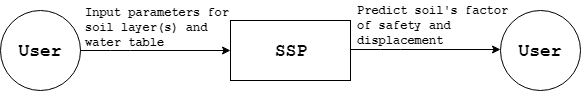
\includegraphics[width=\textwidth]{../../../datafiles/SSP/SystemContextFigure.png}
\caption{System Context}
\label{Figure:sysCtxDiag}
\end{center}
\end{figure}
The responsibilities of the user and the system are as follows:
\begin{itemize}
\item{User Responsibilities}
\begin{itemize}
\item{Provide the input data related to the soil layer(s) and water table (if applicable), ensuring conformation to input data format required by SSP}
\item{Ensure that consistent units are used for input variables}
\item{Ensure required software assumptions (\hyperref[Sec:Assumps]{Section: Assumptions}) are appropriate for the problem to which the user is applying the software}
\end{itemize}
\item{SSP Responsibilities}
\begin{itemize}
\item{Detect data type mismatch, such as a string of characters input instead of a floating point number}
\item{Verify that the inputs satisfy the required physical and other data constraints (\hyperref[Sec:DataConstraints]{Section: Data Constraints})}
\item{Identify the critical slip surface within the possible input range}
\item{Find the factor of safety for the slope}
\item{Find the interslice normal force and shear force along the critical slip surface}
\end{itemize}
\end{itemize}
\subsection{User Characteristics}
\label{Sec:UserChars}
The end user of SSP should have an understanding of undergraduate Level 1 Calculus and Physics, and be familiar with soil and material properties, specifically effective cohesion, effective angle of friction, and unit weight.
\subsection{System Constraints}
\label{Sec:SysConstraints}
The Morgenstern-Price method \cite{morgenstern1965}, which involves dividing the slope into vertical slices, will be used to derive the equations for analysing the slope.
\section{Specific System Description}
\label{Sec:SpecSystDesc}
This section first presents the problem description, which gives a high-level view of the problem to be solved. This is followed by the solution characteristics specification, which presents the assumptions, theories, and definitions that are used.
\subsection{Problem Description}
\label{Sec:ProbDesc}
SSP is a computer program developed to evaluate the factor of safety of a slope's slip surface and identify the critical slip surface of the slope, as well as the interslice normal force and shear force along the critical slip surface. It is intended to be used as an educational tool for introducing slope stability issues, and to facilitate the analysis and design of a safe slope.
\subsubsection{Terminology and Definitions}
\label{Sec:TermDefs}
This subsection provides a list of terms that are used in the subsequent sections and their meaning, with the purpose of reducing ambiguity and making it easier to correctly understand the requirements.
\begin{itemize}
\item[Factor of Safety:]The global stability metric of a slip surface of a slope, defined as the ratio of resistive shear force to mobilized shear force
\item[Slip Surface:]A surface within a slope that has the potential to fail or displace due to load or other forces.
\item[Critical Slip Surface:]Slip surface of the slope that has the lowest factor of safety, and is therefore most likely to experience failure.
\item[Water Table:]The upper boundary of a saturated zone in the ground.
\item[Stress:]Forces that are exerted between planes internal to a larger body subject to external loading.
\item[Strain:]A measure of deformation of a body or plane under stress.
\item[Normal Force:]A force applied perpendicular to the plane of the material.
\item[Shear Force:]A force applied parallel to the plane of the material.
\item[Mobilized Shear Force:]Shear force in the direction of potential motion, thus encouraging motion along the plane.
\item[Resistive Shear Force:]Shear force in the direction opposite to the direction of potential motion, thus hindering motion along the plane.
\item[Effective Forces and Stresses:]The normal force or normal stress carried by the soil skeleton. The total normal force or normal stress is composed of the effective force or stress and the force or stress exerted by water.
\item[Cohesion:]An attractive force between adjacent particles that holds the matter together.
\item[Isotropy:]A condition where the value of a property is independent of the direction in which it is measured.
\item[Plane Strain:]A condition where the resultant stresses in one of the directions of a  three-dimensional material can be approximated as zero. This condition results when a body is constrained to not deform in one direction, or when the length of one dimension of the body dominates the others, to the point where it can be assumed as infinite. Stresses in the direction of the dominant dimension can be approximated as zero.
\end{itemize}
\subsubsection{Physical System Description}
\label{Sec:PhysSyst}
The Physical System Description (PS) of SSP, as shown in \hyperref[Figure:PhysicalSystem]{Fig:PhysicalSystem}, includes the following elements:
\begin{itemize}
\item[PS1:]A slope comprised of one soil layer.
\item[PS2:]A water table, which may or may not exist.
\end{itemize}
\begin{figure}
\begin{center}
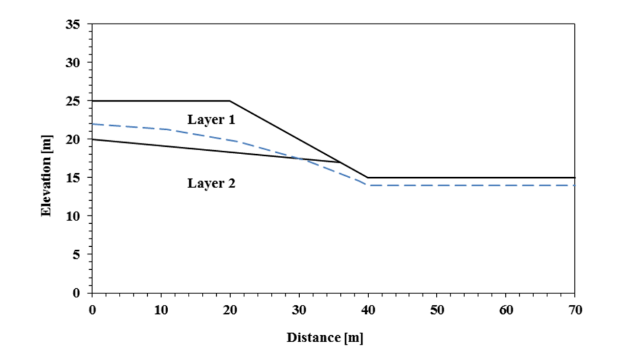
\includegraphics[width=\textwidth]{../../../datafiles/SSP/PhysSyst.png}
\caption{An example slope for analysis by SSP, where the dashed line represents the water table}
\label{Figure:PhysicalSystem}
\end{center}
\end{figure}
Morgenstern-Price analysis \cite{morgenstern1965} of the slope involves representing the slope as a series of vertical slices. As shown in \hyperref[Figure:IndexConvention]{Fig:IndexConvention}, the index $i$ is used to denote a value for a single slice, and an interslice value at a given index $i$ refers to the value between slice $i$ and adjacent slice $i+1$.
\begin{figure}
\begin{center}
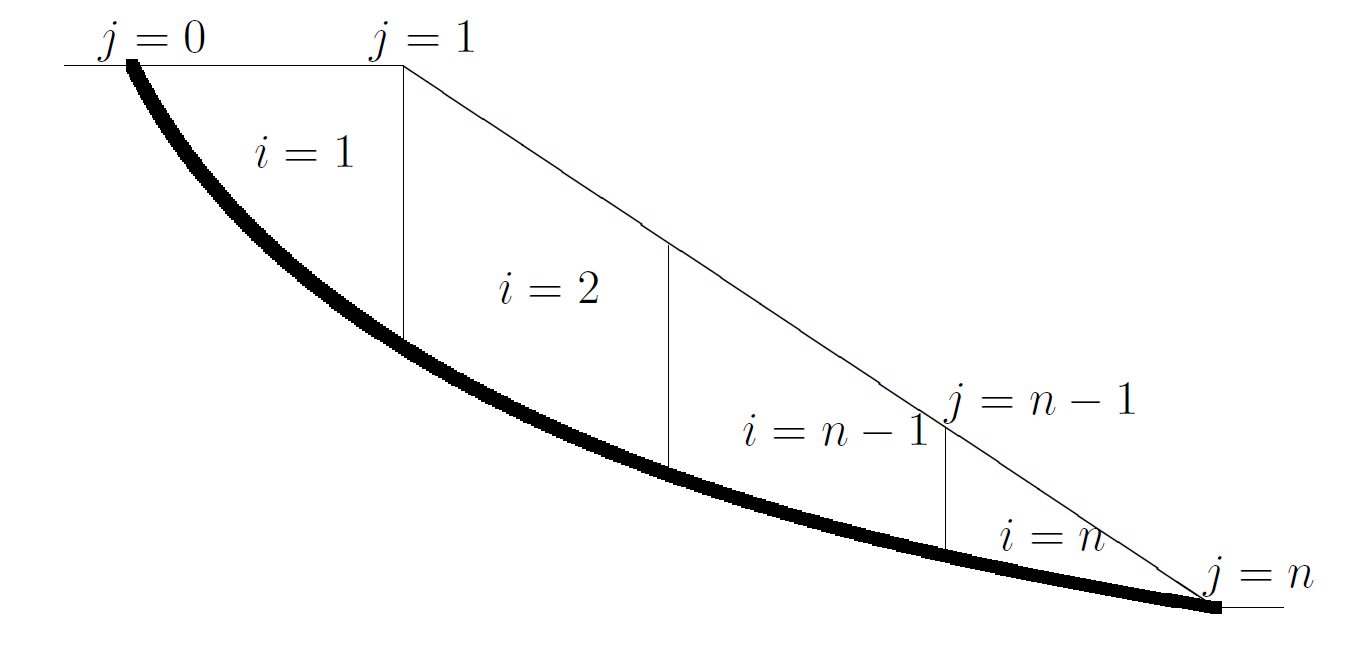
\includegraphics[width=\textwidth]{../../../datafiles/SSP/IndexConvention.png}
\caption{Index convention for slice and interslice values}
\label{Figure:IndexConvention}
\end{center}
\end{figure}
A free body diagram of the forces acting on a slice is displayed in \hyperref[Figure:ForceDiagram]{Fig:ForceDiagram}. The specific forces and symbols will be discussed in detail in \hyperref[Sec:GDs]{Section: General Definitions} and \hyperref[Sec:DDs]{Section: Data Definitions}.
\begin{figure}
\begin{center}
\includegraphics[width=\textwidth]{../../../datafiles/SSP/ForceDiagram.png}
\caption{Free body diagram of forces acting on a slice}
\label{Figure:ForceDiagram}
\end{center}
\end{figure}
\subsubsection{Goal Statements}
\label{Sec:GoalStmt}
Given the shape of the soil mass, the location of the water table, and the material properties of the soil, the goal statements are:
\begin{itemize}
\item[GS1:]Identify the critical slip surface and the corresponding factor of safety.
\item[GS2:]Determine the interslice normal force between each pair of vertical slices of the slope.
\item[GS3:]Determine the interslice shear force between each pair of vertical slices of the slope.
\end{itemize}
\subsection{Solution Characteristics Specification}
\label{Sec:SolCharSpec}
The instance models that govern SSP are presented in \hyperref[Sec:IMs]{Section: Instance Models}. The information to understand the meaning of the instance models and their derivation is also presented, so that the instance models can be verified.
\subsubsection{Assumptions}
\label{Sec:Assumps}
This section simplifies the original problem and helps in developing the theoretical model by filling in the missing information for the physical system. The numbers given in the square brackets refer to the Theoretical Models \hyperref[Sec:TMs]{Section: Theoretical Models}, General Definitions \hyperref[Sec:GDs]{Section: General Definitions}, Data Definitions \hyperref[Sec:DDs]{Section: Data Definitions}, Instance Models \hyperref[Sec:IMs]{Section: Instance Models}, Likely Changes \hyperref[Sec:LCs]{Section: Likely Changes}, or Unlikely Changes \hyperref[Sec:UCs]{Section: Unlikely Changes}, in which the respective assumption is used.
\begin{itemize}
\item[Slip-Surface-Concave:\phantomsection\label{assumpSSC}]The slip surface is concave with respect to the slope surface. The (${x_{slip}}$, ${y_{slip}}$) coordinates of a slip surface follow a concave up function. \hyperref[IM:crtSlpId]{IM: crtSlpId}.
\item[Factor-of-Safety:\phantomsection\label{assumpFOS}]The factor of safety is assumed to be constant across the entire slip surface. \hyperref[GD:mobShr]{GD: mobShr}.
\item[Soil-Layer-Homogeneous:\phantomsection\label{assumpSLH}]The soil mass is homogeneous, with consistent soil properties throughout. \hyperref[GD:resShr]{GD: resShr} \hyperref[DD:sliceWght]{DD: sliceWght} \hyperref[LC_inhomogeneous]{LC: Calculate-Inhomogeneous-Soil-Layers}.
\item[Soil-Properties:\phantomsection\label{assumpSP}]The soil properties are independent of dry or saturated conditions, with the exception of unit weight. \hyperref[GD:resShr]{GD: resShr}.
\item[Soil-Layers-Isotropic:\phantomsection\label{assumpSLI}]The soil mass is treated as if the effective cohesion and effective angle of friction are isotropic properties. \hyperref[GD:resShr]{GD: resShr}.
\item[Interslice-Norm-Shear-Forces-Linear:\phantomsection\label{assumpINSFL}]Following the assumption of Morgenstern and Price (\cite{morgenstern1965}), interslice normal force and interslice shear force have a proportional relationship, depending on a proportionality constant ($λ$) and a function ($f$) describing variation depending on $x$ position. \hyperref[IM:nrmShrFor]{IM: nrmShrFor} \hyperref[GD:normShrR]{GD: normShrR} \hyperref[IM:fctSfty]{IM: fctSfty} \hyperref[UC_normshearlinear]{UC: Normal-And-Shear-Linear-Only}.
\item[Plane-Strain-Conditions:\phantomsection\label{assumpPSC}]The slope and slip surface extends far into and out of the geometry ($z$ coordinate). This implies plane strain conditions, making 2D analysis appropriate. \hyperref[GD:resShr]{GD: resShr} \hyperref[GD:effNormF]{GD: effNormF}.
\item[Effective-Norm-Stress-Large:\phantomsection\label{assumpENSL}]The effective normal stress is large enough that the shear strength to effective normal stress relationship can be approximated as a linear relationship. \hyperref[TM:equilibrium]{TM: equilibrium} \hyperref[UC_2donly]{UC: 2D-Analysis-Only}.
\item[Surface-Base-Slice-between-Interslice-Straight-Lines:\phantomsection\label{assumpSBSBISL}]The surface and base of a slice are approximated as straight lines. \hyperref[TM:mcShrStrgth]{TM: mcShrStrgth} \hyperref[DD:slcHeight]{DD: slcHeight} \hyperref[DD:angleB]{DD: angleB} \hyperref[DD:angleA]{DD: angleA} \hyperref[DD:sliceWght]{DD: sliceWght} \hyperref[DD:surfWtrF]{DD: surfWtrF} \hyperref[DD:baseWtrF]{DD: baseWtrF}.
\item[Edge-Slices:\phantomsection\label{assumpES}]The interslice forces at the 0th and $n$th interslice interfaces are zero. \hyperref[IM:nrmShrFor]{IM: nrmShrFor} \hyperref[IM:intsliceFs]{IM: intsliceFs} \hyperref[IM:fctSfty]{IM: fctSfty}.
\item[Seismic-Force:\phantomsection\label{assumpSF}]There is no seismic force acting on the slope. \hyperref[IM:nrmShrFor]{IM: nrmShrFor} \hyperref[IM:fctSfty]{IM: fctSfty} \hyperref[LC_seismic]{LC: Calculate-Seismic-Force}.
\item[Surface-Load:\phantomsection\label{assumpSL}]There is no imposed surface load, and therefore no external force, acting on the slope. \hyperref[IM:nrmShrFor]{IM: nrmShrFor} \hyperref[IM:fctSfty]{IM: fctSfty} \hyperref[LC_external]{LC: Calculate-External-Force}.
\end{itemize}
\subsubsection{Theoretical Models}
\label{Sec:TMs}
This section focuses on the general equations and laws that SSP is based on.
\par~

\noindent \begin{minipage}{\textwidth}
\begin{tabular}{p{0.2\textwidth} p{0.73\textwidth}}
\toprule \textbf{Refname} & \textbf{TM:factOfSafety}
\phantomsection 
\label{TM:factOfSafety}
\\ \midrule \\
Label & Factor of safety
        \\ \midrule \\
        Equation & \begin{displaymath}
                   {F_{S}}=\frac{P}{S}
                   \end{displaymath}
                   \\ \midrule \\
                   Description & \begin{symbDescription}
                                 \item{${F_{S}}$ is the factor of safety (Unitless)}
                                 \item{$P$ is the resistive shear force ($\frac{\text{N}}{\text{m}}$)}
                                 \item{$S$ is the mobilized shear force ($\frac{\text{N}}{\text{m}}$)}
                                 \end{symbDescription}
                                 \\ \midrule \\
                                 Source & \cite{fredlund1977}
                                          \\ \midrule \\
                                          RefBy & \hyperref[GD:mobShr]{GD: mobShr}.
\\ \bottomrule \end{tabular}
\end{minipage}
\par~

\noindent \begin{minipage}{\textwidth}
\begin{tabular}{p{0.2\textwidth} p{0.73\textwidth}}
\toprule \textbf{Refname} & \textbf{TM:equilibrium}
\phantomsection 
\label{TM:equilibrium}
\\ \midrule \\
Label & Equilibrium
        \\ \midrule \\
        Equation & \begin{displaymath}
                   \displaystyle\sum{{F_{x}}}=\displaystyle\sum{{F_{y}}}=\displaystyle\sum{M}=0
                   \end{displaymath}
                   \\ \midrule \\
                   Description & \begin{symbDescription}
                                 \item{${F_{x}}$ is the x-component of the net force (N)}
                                 \item{${F_{y}}$ is the y-component of the net force (N)}
                                 \item{$M$ is the net moment (Nm)}
                                 \end{symbDescription}
                                 \\ \midrule \\
                                 Notes & For a body in static equilibrium, the net forces and net moments acting on the body will cancel out. Assuming a 2D problem (\hyperref[assumpENSL]{A: Effective-Norm-Stress-Large}), the x-component of the net force ${F_{x}}$ and y-component of the net force ${F_{y}}$ will be equal to $0$. All forces and their distance from the chosen point of rotation will create a net moment equal to $0$.
                                         \\ \midrule \\
                                         Source & \cite{fredlund1977}
                                                  \\ \midrule \\
                                                  RefBy & \hyperref[GD:normForcEq]{GD: normForcEq} \hyperref[GD:momentEql]{GD: momentEql} \hyperref[GD:bsShrFEq]{GD: bsShrFEq}.
\\ \bottomrule \end{tabular}
\end{minipage}
\par~

\noindent \begin{minipage}{\textwidth}
\begin{tabular}{p{0.2\textwidth} p{0.73\textwidth}}
\toprule \textbf{Refname} & \textbf{TM:mcShrStrgth}
\phantomsection 
\label{TM:mcShrStrgth}
\\ \midrule \\
Label & Mohr-Coulumb shear strength
        \\ \midrule \\
        Equation & \begin{displaymath}
                   τ={σ_{N}}' \tan\left(φ'\right)+c'
                   \end{displaymath}
                   \\ \midrule \\
                   Description & \begin{symbDescription}
                                 \item{$τ$ is the shear strength (Pa)}
                                 \item{${σ_{N}}'$ is the effective normal stress (Pa)}
                                 \item{$φ'$ is the effective angle of friction (${}^{\circ}$)}
                                 \item{$c'$ is the effective cohesion (Pa)}
                                 \end{symbDescription}
                                 \\ \midrule \\
                                 Notes & In this model the shear strength $τ$ is proportional to the product of the effective normal stress ${σ_{N}}'$ on the plane with its static friction in the angular form $\tan\left(φ'\right)$. The $τ$ versus ${σ_{N}}'$ relationship is not truly linear, but assuming the effective normal force is strong enough, it can be approximated with a linear fit (\hyperref[assumpSBSBISL]{A: Surface-Base-Slice-between-Interslice-Straight-Lines}) where the effective cohesion $c'$ represents the $τ$ intercept of the fitted line.
                                         \\ \midrule \\
                                         Source & \cite{fredlund1977}
                                                  \\ \midrule \\
                                                  RefBy & \hyperref[GD:resShr]{GD: resShr}.
\\ \bottomrule \end{tabular}
\end{minipage}
\par~

\noindent \begin{minipage}{\textwidth}
\begin{tabular}{p{0.2\textwidth} p{0.73\textwidth}}
\toprule \textbf{Refname} & \textbf{TM:effStress}
\phantomsection 
\label{TM:effStress}
\\ \midrule \\
Label & Effective stress
        \\ \midrule \\
        Equation & \begin{displaymath}
                   σ'=σ-u
                   \end{displaymath}
                   \\ \midrule \\
                   Description & \begin{symbDescription}
                                 \item{$σ'$ is the effective stress (Pa)}
                                 \item{$σ$ is the total stress (Pa)}
                                 \item{$u$ is the pore pressure (Pa)}
                                 \end{symbDescription}
                                 \\ \midrule \\
                                 Notes & $σ$ is defined in \hyperref[DD:stress]{DD: stress}.
                                         \\ \midrule \\
                                         Source & \cite{fredlund1977}
                                                  \\ \midrule \\
                                                  RefBy & \hyperref[GD:effNormF]{GD: effNormF}.
\\ \bottomrule \end{tabular}
\end{minipage}
\subsubsection{General Definitions}
\label{Sec:GDs}
This section collects the laws and equations that will be used to build the instance models.
\par~

\noindent \begin{minipage}{\textwidth}
\begin{tabular}{p{0.2\textwidth} p{0.73\textwidth}}
\toprule \textbf{Refname} & \textbf{GD:normForcEq}
\phantomsection 
\label{GD:normForcEq}
\\ \midrule \\
Label & Normal force equilibrium
        \\ \midrule \\
        Units & $\frac{\text{N}}{\text{m}}$
                \\ \midrule \\
                Equation & \begin{displaymath}
                           N_{i}=\left(W_{i}-X_{i-1}+X_{i}+{U_{t,i}} \cos\left(β_{i}\right)+Q_{i} \cos\left(ω_{i}\right)\right) \cos\left(α_{i}\right)+\left(-{K_{c}} W_{i}-G_{i}+G_{i-1}-H_{i}+H_{i-1}+{U_{t,i}} \sin\left(β_{i}\right)+Q_{i} \sin\left(ω_{i}\right)\right) \sin\left(α_{i}\right)
                           \end{displaymath}
                           \\ \midrule \\
                           Description & \begin{symbDescription}
                                         \item{$N$ is the normal force ($\frac{\text{N}}{\text{m}}$)}
                                         \item{$i$ is the index (Unitless)}
                                         \item{$W$ is the weight ($\frac{\text{N}}{\text{m}}$)}
                                         \item{$X$ is the interslice shear force ($\frac{\text{N}}{\text{m}}$)}
                                         \item{${U_{t}}$ is the surface hydrostatic force ($\frac{\text{N}}{\text{m}}$)}
                                         \item{$β$ is the surface angle (${}^{\circ}$)}
                                         \item{$Q$ is the external force ($\frac{\text{N}}{\text{m}}$)}
                                         \item{$ω$ is the imposed load angle (${}^{\circ}$)}
                                         \item{$α$ is the base angle (${}^{\circ}$)}
                                         \item{${K_{c}}$ is the seismic coefficient (Unitless)}
                                         \item{$G$ is the interslice normal force ($\frac{\text{N}}{\text{m}}$)}
                                         \item{$H$ is the interslice normal water force  ($\frac{\text{N}}{\text{m}}$)}
                                         \end{symbDescription}
                                         \\ \midrule \\
                                         Notes & This equation satisfies \hyperref[TM:equilibrium]{TM: equilibrium} in the normal direction. $W$ is defined in \hyperref[DD:sliceWght]{DD: sliceWght}, ${U_{t}}$ is defined in \hyperref[DD:surfWtrF]{DD: surfWtrF}, $β$ is defined in \hyperref[DD:angleB]{DD: angleB}, and $α$ is defined in \hyperref[DD:angleA]{DD: angleA}.
                                                 \\ \midrule \\
                                                 Source & \cite{chen2005}
                                                          \\ \midrule \\
                                                          RefBy & \hyperref[IM:fctSfty]{IM: fctSfty}.
\\ \bottomrule \end{tabular}
\end{minipage}
Normal force equilibrium is derived from the free body diagram of \hyperref[Figure:ForceDiagram]{Fig:ForceDiagram} in \hyperref[Sec:PhysSyst]{Section: Physical System Description}.
\par~

\noindent \begin{minipage}{\textwidth}
\begin{tabular}{p{0.2\textwidth} p{0.73\textwidth}}
\toprule \textbf{Refname} & \textbf{GD:bsShrFEq}
\phantomsection 
\label{GD:bsShrFEq}
\\ \midrule \\
Label & Base shear force equilibrium
        \\ \midrule \\
        Units & $\frac{\text{N}}{\text{m}}$
                \\ \midrule \\
                Equation & \begin{displaymath}
                           S_{i}=\left(W_{i}-X_{i-1}+X_{i}+{U_{t,i}} \cos\left(β_{i}\right)+Q_{i} \cos\left(ω_{i}\right)\right) \sin\left(α_{i}\right)-\left(-{K_{c}} W_{i}-G_{i}+G_{i-1}-H_{i}+H_{i-1}+{U_{t,i}} \sin\left(β_{i}\right)+Q_{i} \sin\left(ω_{i}\right)\right) \cos\left(α_{i}\right)
                           \end{displaymath}
                           \\ \midrule \\
                           Description & \begin{symbDescription}
                                         \item{$S$ is the mobilized shear force ($\frac{\text{N}}{\text{m}}$)}
                                         \item{$i$ is the index (Unitless)}
                                         \item{$W$ is the weight ($\frac{\text{N}}{\text{m}}$)}
                                         \item{$X$ is the interslice shear force ($\frac{\text{N}}{\text{m}}$)}
                                         \item{${U_{t}}$ is the surface hydrostatic force ($\frac{\text{N}}{\text{m}}$)}
                                         \item{$β$ is the surface angle (${}^{\circ}$)}
                                         \item{$Q$ is the external force ($\frac{\text{N}}{\text{m}}$)}
                                         \item{$ω$ is the imposed load angle (${}^{\circ}$)}
                                         \item{$α$ is the base angle (${}^{\circ}$)}
                                         \item{${K_{c}}$ is the seismic coefficient (Unitless)}
                                         \item{$G$ is the interslice normal force ($\frac{\text{N}}{\text{m}}$)}
                                         \item{$H$ is the interslice normal water force  ($\frac{\text{N}}{\text{m}}$)}
                                         \end{symbDescription}
                                         \\ \midrule \\
                                         Notes & This equation satisfies \hyperref[TM:equilibrium]{TM: equilibrium} in the shear direction. $W$ is defined in \hyperref[DD:sliceWght]{DD: sliceWght}, ${U_{t}}$ is defined in \hyperref[DD:surfWtrF]{DD: surfWtrF}, $β$ is defined in \hyperref[DD:angleB]{DD: angleB}, and $α$ is defined in \hyperref[DD:angleA]{DD: angleA}.
                                                 \\ \midrule \\
                                                 Source & \cite{chen2005}
                                                          \\ \midrule \\
                                                          RefBy & \hyperref[IM:fctSfty]{IM: fctSfty}.
\\ \bottomrule \end{tabular}
\end{minipage}
Base shear force equilibrium is derived from the free body diagram of \hyperref[Figure:ForceDiagram]{Fig:ForceDiagram} in \hyperref[Sec:PhysSyst]{Section: Physical System Description}.
\par~

\noindent \begin{minipage}{\textwidth}
\begin{tabular}{p{0.2\textwidth} p{0.73\textwidth}}
\toprule \textbf{Refname} & \textbf{GD:resShr}
\phantomsection 
\label{GD:resShr}
\\ \midrule \\
Label & Resistive shear force
        \\ \midrule \\
        Units & $\frac{\text{N}}{\text{m}}$
                \\ \midrule \\
                Equation & \begin{displaymath}
                           P_{i}={N'}_{i} \tan\left({φ'}_{i}\right)+{c'}_{i} {ℓ_{b,i}}
                           \end{displaymath}
                           \\ \midrule \\
                           Description & \begin{symbDescription}
                                         \item{$P$ is the resistive shear force ($\frac{\text{N}}{\text{m}}$)}
                                         \item{$i$ is the index (Unitless)}
                                         \item{$N'$ is the effective normal force ($\frac{\text{N}}{\text{m}}$)}
                                         \item{$φ'$ is the effective angle of friction (${}^{\circ}$)}
                                         \item{$c'$ is the effective cohesion (Pa)}
                                         \item{${ℓ_{b}}$ is the total base length of a slice (m)}
                                         \end{symbDescription}
                                         \\ \midrule \\
                                         Notes & ${ℓ_{b}}$ is defined in \hyperref[DD:lengthLb]{DD: lengthLb}.
                                                 \\ \midrule \\
                                                 Source & \cite{chen2005}
                                                          \\ \midrule \\
                                                          RefBy & \hyperref[GD:mobShr]{GD: mobShr}.
\\ \bottomrule \end{tabular}
\end{minipage}
Derived by substituting \hyperref[DD:stress]{DD: stress} into the Mohr-Coulomb shear strength, \hyperref[TM:mcShrStrgth]{TM: mcShrStrgth}, and multiplying both sides of the equation by the area of the slice in the shear-$z$ plane. Since the slope is assumed to extend infinitely in the $z$-direction (\hyperref[assumpPSC]{A: Plane-Strain-Conditions}), the resulting forces are expressed per metre in the $z$-direction. The effective angle of friction $φ'$ and the effective cohesion $c'$ are not indexed by $i$ becaused they are assumed to be isotropic (\hyperref[assumpSLI]{A: Soil-Layers-Isotropic}) and the soil is assumed to be homogeneous, with constant soil properties throughout (\hyperref[assumpSLH]{A: Soil-Layer-Homogeneous}, \hyperref[assumpSP]{A: Soil-Properties}).
\par~

\noindent \begin{minipage}{\textwidth}
\begin{tabular}{p{0.2\textwidth} p{0.73\textwidth}}
\toprule \textbf{Refname} & \textbf{GD:mobShr}
\phantomsection 
\label{GD:mobShr}
\\ \midrule \\
Label & Mobilized shear force
        \\ \midrule \\
        Units & $\frac{\text{N}}{\text{m}}$
                \\ \midrule \\
                Equation & \begin{displaymath}
                           S_{i}=\frac{P_{i}}{{F_{S}}}=\frac{{N'}_{i} \tan\left({φ'}_{i}\right)+{c'}_{i} {ℓ_{b,i}}}{{F_{S}}}
                           \end{displaymath}
                           \\ \midrule \\
                           Description & \begin{symbDescription}
                                         \item{$S$ is the mobilized shear force ($\frac{\text{N}}{\text{m}}$)}
                                         \item{$i$ is the index (Unitless)}
                                         \item{$P$ is the resistive shear force ($\frac{\text{N}}{\text{m}}$)}
                                         \item{${F_{S}}$ is the factor of safety (Unitless)}
                                         \item{$N'$ is the effective normal force ($\frac{\text{N}}{\text{m}}$)}
                                         \item{$φ'$ is the effective angle of friction (${}^{\circ}$)}
                                         \item{$c'$ is the effective cohesion (Pa)}
                                         \item{${ℓ_{b}}$ is the total base length of a slice (m)}
                                         \end{symbDescription}
                                         \\ \midrule \\
                                         Notes & ${ℓ_{b}}$ is defined in \hyperref[DD:lengthLb]{DD: lengthLb}.
                                                 \\ \midrule \\
                                                 Source & \cite{chen2005}
                                                          \\ \midrule \\
                                                          RefBy & \hyperref[IM:fctSfty]{IM: fctSfty}.
\\ \bottomrule \end{tabular}
\end{minipage}
Mobilized shear force is derived by dividing the definition of the $P$ from \hyperref[GD:resShr]{GD: resShr}. by the definition of the factor of safety from \hyperref[TM:factOfSafety]{TM: factOfSafety}. The factor of safety ${F_{S}}$ is not indexed by $i$ because it is assumed to be constant for the entire slip surface (\hyperref[assumpFOS]{A: Factor-of-Safety}).
\par~

\noindent \begin{minipage}{\textwidth}
\begin{tabular}{p{0.2\textwidth} p{0.73\textwidth}}
\toprule \textbf{Refname} & \textbf{GD:effNormF}
\phantomsection 
\label{GD:effNormF}
\\ \midrule \\
Label & Effective normal force
        \\ \midrule \\
        Units & $\frac{\text{N}}{\text{m}}$
                \\ \midrule \\
                Equation & \begin{displaymath}
                           {N'}_{i}=N_{i}-{U_{b,i}}
                           \end{displaymath}
                           \\ \midrule \\
                           Description & \begin{symbDescription}
                                         \item{$N'$ is the effective normal force ($\frac{\text{N}}{\text{m}}$)}
                                         \item{$i$ is the index (Unitless)}
                                         \item{$N$ is the normal force ($\frac{\text{N}}{\text{m}}$)}
                                         \item{${U_{b}}$ is the base hydrostatic force ($\frac{\text{N}}{\text{m}}$)}
                                         \end{symbDescription}
                                         \\ \midrule \\
                                         Notes & ${U_{b}}$ is defined in \hyperref[DD:baseWtrF]{DD: baseWtrF}.
                                                 \\ \midrule \\
                                                 Source & \cite{chen2005}
                                                          \\ \midrule \\
                                                          RefBy & 
\\ \bottomrule \end{tabular}
\end{minipage}
Derived by substituting \hyperref[DD:stress]{DD: stress} into \hyperref[TM:effStress]{TM: effStress} and multiplying both sides of the equation by the the area of the slice in the shear-$z$ plane. Since the slope is assumed to extend infinitely in the $z$-direction (\hyperref[assumpPSC]{A: Plane-Strain-Conditions}), the resulting forces are expressed per metre in the $z$-direction.
\par~

\noindent \begin{minipage}{\textwidth}
\begin{tabular}{p{0.2\textwidth} p{0.73\textwidth}}
\toprule \textbf{Refname} & \textbf{GD:resShearWO}
\phantomsection 
\label{GD:resShearWO}
\\ \midrule \\
Label & Resistive shear force, without interslice normal and shear forces
        \\ \midrule \\
        Units & $\frac{\text{N}}{\text{m}}$
                \\ \midrule \\
                Equation & \begin{displaymath}
                           R_{i}=\left(\left(W_{i}+{U_{t,i}} \cos\left(β_{i}\right)\right) \cos\left(α_{i}\right)+\left(-H_{i}+H_{i-1}+{U_{t,i}} \sin\left(β_{i}\right)\right) \sin\left(α_{i}\right)-{U_{b,i}}\right) \tan\left({φ'}_{i}\right)+{c'}_{i} {ℓ_{b,i}}
                           \end{displaymath}
                           \\ \midrule \\
                           Description & \begin{symbDescription}
                                         \item{$R$ is the resistive shear force without the influence of interslice forces ($\frac{\text{N}}{\text{m}}$)}
                                         \item{$i$ is the index (Unitless)}
                                         \item{$W$ is the weight ($\frac{\text{N}}{\text{m}}$)}
                                         \item{${U_{t}}$ is the surface hydrostatic force ($\frac{\text{N}}{\text{m}}$)}
                                         \item{$β$ is the surface angle (${}^{\circ}$)}
                                         \item{$α$ is the base angle (${}^{\circ}$)}
                                         \item{$H$ is the interslice normal water force  ($\frac{\text{N}}{\text{m}}$)}
                                         \item{${U_{b}}$ is the base hydrostatic force ($\frac{\text{N}}{\text{m}}$)}
                                         \item{$φ'$ is the effective angle of friction (${}^{\circ}$)}
                                         \item{$c'$ is the effective cohesion (Pa)}
                                         \item{${ℓ_{b}}$ is the total base length of a slice (m)}
                                         \end{symbDescription}
                                         \\ \midrule \\
                                         Notes & $W$ is defined in \hyperref[DD:sliceWght]{DD: sliceWght}, ${U_{t}}$ is defined in \hyperref[DD:surfWtrF]{DD: surfWtrF}, $β$ is defined in \hyperref[DD:angleB]{DD: angleB}, $α$ is defined in \hyperref[DD:angleA]{DD: angleA}, $H$ is defined in \hyperref[DD:intersliceWtrF]{DD: intersliceWtrF}, ${U_{b}}$ is defined in \hyperref[DD:baseWtrF]{DD: baseWtrF}, and ${ℓ_{b}}$ is defined in \hyperref[DD:lengthLb]{DD: lengthLb}.
                                                 \\ \midrule \\
                                                 Source & \cite{chen2005}
                                                          \\ \midrule \\
                                                          RefBy & \hyperref[IM:intsliceFs]{IM: intsliceFs} \hyperref[IM:fctSfty]{IM: fctSfty} \hyperref[IM:fctSfty]{IM: fctSfty} \hyperref[IM:fctSfty]{IM: fctSfty}.
\\ \bottomrule \end{tabular}
\end{minipage}
\par~

\noindent \begin{minipage}{\textwidth}
\begin{tabular}{p{0.2\textwidth} p{0.73\textwidth}}
\toprule \textbf{Refname} & \textbf{GD:mobShearWO}
\phantomsection 
\label{GD:mobShearWO}
\\ \midrule \\
Label & Mobilized shear force, without interslice normal and shear forces
        \\ \midrule \\
        Units & $\frac{\text{N}}{\text{m}}$
                \\ \midrule \\
                Equation & \begin{displaymath}
                           T_{i}=\left(W_{i}+{U_{t,i}} \cos\left(β_{i}\right)\right) \sin\left(α_{i}\right)-\left(-H_{i}+H_{i-1}+{U_{t,i}} \sin\left(β_{i}\right)\right) \cos\left(α_{i}\right)
                           \end{displaymath}
                           \\ \midrule \\
                           Description & \begin{symbDescription}
                                         \item{$T$ is the mobilized shear force without the influence of interslice forces ($\frac{\text{N}}{\text{m}}$)}
                                         \item{$i$ is the index (Unitless)}
                                         \item{$W$ is the weight ($\frac{\text{N}}{\text{m}}$)}
                                         \item{${U_{t}}$ is the surface hydrostatic force ($\frac{\text{N}}{\text{m}}$)}
                                         \item{$β$ is the surface angle (${}^{\circ}$)}
                                         \item{$α$ is the base angle (${}^{\circ}$)}
                                         \item{$H$ is the interslice normal water force  ($\frac{\text{N}}{\text{m}}$)}
                                         \end{symbDescription}
                                         \\ \midrule \\
                                         Notes & $W$ is defined in \hyperref[DD:sliceWght]{DD: sliceWght}, ${U_{t}}$ is defined in \hyperref[DD:surfWtrF]{DD: surfWtrF}, $β$ is defined in \hyperref[DD:angleB]{DD: angleB}, $α$ is defined in \hyperref[DD:angleA]{DD: angleA}, and $H$ is defined in \hyperref[DD:intersliceWtrF]{DD: intersliceWtrF}.
                                                 \\ \midrule \\
                                                 Source & \cite{chen2005}
                                                          \\ \midrule \\
                                                          RefBy & \hyperref[IM:intsliceFs]{IM: intsliceFs} \hyperref[IM:fctSfty]{IM: fctSfty} \hyperref[IM:fctSfty]{IM: fctSfty}.
\\ \bottomrule \end{tabular}
\end{minipage}
\par~

\noindent \begin{minipage}{\textwidth}
\begin{tabular}{p{0.2\textwidth} p{0.73\textwidth}}
\toprule \textbf{Refname} & \textbf{GD:normShrR}
\phantomsection 
\label{GD:normShrR}
\\ \midrule \\
Label & Interslice normal and shear force proportionality
        \\ \midrule \\
        Units & $\frac{\text{N}}{\text{m}}$
                \\ \midrule \\
                Equation & \begin{displaymath}
                           X=λ f G
                           \end{displaymath}
                           \\ \midrule \\
                           Description & \begin{symbDescription}
                                         \item{$X$ is the interslice shear force ($\frac{\text{N}}{\text{m}}$)}
                                         \item{$λ$ is the proportionality constant (Unitless)}
                                         \item{$f$ is the interslice normal to shear force ratio variation function (Unitless)}
                                         \item{$G$ is the interslice normal force ($\frac{\text{N}}{\text{m}}$)}
                                         \end{symbDescription}
                                         \\ \midrule \\
                                         Notes & Mathematical representation of the primary assumption for the Morgenstern-Price method (\hyperref[assumpINSFL]{A: Interslice-Norm-Shear-Forces-Linear}). $f$ is defined in \hyperref[DD:ratioVariation]{DD: ratioVariation}.
                                                 \\ \midrule \\
                                                 Source & \cite{chen2005}
                                                          \\ \midrule \\
                                                          RefBy & \hyperref[IM:nrmShrFor]{IM: nrmShrFor} \hyperref[IM:fctSfty]{IM: fctSfty}.
\\ \bottomrule \end{tabular}
\end{minipage}
\par~

\noindent \begin{minipage}{\textwidth}
\begin{tabular}{p{0.2\textwidth} p{0.73\textwidth}}
\toprule \textbf{Refname} & \textbf{GD:momentEql}
\phantomsection 
\label{GD:momentEql}
\\ \midrule \\
Label & Moment equilibrium
        \\ \midrule \\
        Units & N
                \\ \midrule \\
                Equation & \begin{displaymath}
                           0=-G_{i} \left({h_{z,i}}-\frac{b_{i}}{2} \tan\left(α_{i}\right)\right)+G_{i-1} \left({h_{z,i-1}}+\frac{b_{i}}{2} \tan\left(α_{i}\right)\right)-H_{i} \left({h_{z,w,i}}-\frac{b_{i}}{2} \tan\left(α_{i}\right)\right)+H_{i-1} \left({h_{z,w,i-1}}+\frac{b_{i}}{2} \tan\left(α_{i}\right)\right)-\frac{b_{i}}{2} \left(X_{i}+X_{i-1}\right)+\frac{{K_{c}} W_{i} h_{i}}{2}-{U_{t,i}} \sin\left(β_{i}\right) h_{i}-Q_{i} \sin\left(ω_{i}\right) h_{i}
                           \end{displaymath}
                           \\ \midrule \\
                           Description & \begin{symbDescription}
                                         \item{$G$ is the interslice normal force ($\frac{\text{N}}{\text{m}}$)}
                                         \item{$i$ is the index (Unitless)}
                                         \item{${h_{z}}$ is the height of center of slice (m)}
                                         \item{$b$ is the base width of a slice (m)}
                                         \item{$α$ is the base angle (${}^{\circ}$)}
                                         \item{$H$ is the interslice normal water force  ($\frac{\text{N}}{\text{m}}$)}
                                         \item{${h_{z,w}}$ is the height halfway to water table (m)}
                                         \item{$X$ is the interslice shear force ($\frac{\text{N}}{\text{m}}$)}
                                         \item{${K_{c}}$ is the seismic coefficient (Unitless)}
                                         \item{$W$ is the weight ($\frac{\text{N}}{\text{m}}$)}
                                         \item{$h$ is the y-direction height of a slice (m)}
                                         \item{${U_{t}}$ is the surface hydrostatic force ($\frac{\text{N}}{\text{m}}$)}
                                         \item{$β$ is the surface angle (${}^{\circ}$)}
                                         \item{$Q$ is the external force ($\frac{\text{N}}{\text{m}}$)}
                                         \item{$ω$ is the imposed load angle (${}^{\circ}$)}
                                         \end{symbDescription}
                                         \\ \midrule \\
                                         Notes & This equation satisfies \hyperref[TM:equilibrium]{TM: equilibrium} for the net moment. $b$ is defined in \hyperref[DD:lengthB]{DD: lengthB}, $α$ is defined in \hyperref[DD:angleA]{DD: angleA}, $W$ is defined in \hyperref[DD:sliceWght]{DD: sliceWght}, $h$ is defined in \hyperref[DD:slcHeight]{DD: slcHeight}, ${U_{t}}$ is defined in \hyperref[DD:surfWtrF]{DD: surfWtrF}, and $β$ is defined in \hyperref[DD:angleB]{DD: angleB}.
                                                 \\ \midrule \\
                                                 Source & \cite{chen2005}
                                                          \\ \midrule \\
                                                          RefBy & \hyperref[IM:nrmShrFor]{IM: nrmShrFor}.
\\ \bottomrule \end{tabular}
\end{minipage}
Moment equilibrium is derived from the free body diagram of \hyperref[Sec:PhysSyst]{Section: Physical System Description}.
\subsubsection{Data Definitions}
\label{Sec:DDs}
This section collects and defines all the data needed to build the instance models.
\par~

\noindent \begin{minipage}{\textwidth}
\begin{tabular}{p{0.2\textwidth} p{0.73\textwidth}}
\toprule \textbf{Refname} & \textbf{DD:sliceWght}
\phantomsection 
\label{DD:sliceWght}
\\ \midrule \\
Label & Weight
        \\ \midrule \\
        Symbol & $W$
                 \\ \midrule \\
                 Units & $\frac{\text{N}}{\text{m}}$
                         \\ \midrule \\
                         Equation & \begin{displaymath}
                                    W=\frac{1}{2} \left({{W^{L}}}_{i}+{{W^{R}}}_{i}\right)
                                    \end{displaymath}
                                    \\ \midrule \\
                                    Description & \begin{symbDescription}
                                                  \item{$W$ is the weight ($\frac{\text{N}}{\text{m}}$)}
                                                  \item{${W^{L}}$ is the left weight of a slice ($\frac{\text{N}}{\text{m}}$)}
                                                  \item{$i$ is the index (Unitless)}
                                                  \item{${W^{R}}$ is the right weight of a slice ($\frac{\text{N}}{\text{m}}$)}
                                                  \end{symbDescription}
                                                  \\ \midrule \\
                                                  Notes & This equation is based on the assumption that the surface and the base of a slice are straight lines (\hyperref[assumpSBSBISL]{A: Surface-Base-Slice-between-Interslice-Straight-Lines}). The soil dry unit weight $γ$ and the soil saturated unit weight ${γ_{Sat}}$ are not indexed by $i$ because the soil is assumed to be homogeneous, with constant soil properties throughout (\hyperref[assumpSLH]{A: Soil-Layer-Homogeneous}). ${W^{L}}$ is defined in \hyperref[DD:slcWghtRDD]{DD: slcWghtRDD} and ${W^{R}}$ is defined in \hyperref[DD:slcWghtRDD]{DD: slcWghtRDD}.
                                                          \\ \midrule \\
                                                          Source & \cite{fredlund1977}
                                                                   \\ \midrule \\
                                                                   RefBy & \hyperref[GD:resShearWO]{GD: resShearWO} \hyperref[GD:normForcEq]{GD: normForcEq} \hyperref[GD:momentEql]{GD: momentEql} \hyperref[GD:mobShearWO]{GD: mobShearWO} \hyperref[GD:bsShrFEq]{GD: bsShrFEq}.
\\ \bottomrule \end{tabular}
\end{minipage}
\par~

\noindent \begin{minipage}{\textwidth}
\begin{tabular}{p{0.2\textwidth} p{0.73\textwidth}}
\toprule \textbf{Refname} & \textbf{DD:baseWtrF}
\phantomsection 
\label{DD:baseWtrF}
\\ \midrule \\
Label & Base hydrostatic force
        \\ \midrule \\
        Symbol & ${U_{b}}$
                 \\ \midrule \\
                 Units & $\frac{\text{N}}{\text{m}}$
                         \\ \midrule \\
                         Equation & \begin{displaymath}
                                    {U_{b}}=\frac{1}{2} \left({{U^{L}}_{b,i}}+{{U^{R}}_{b,i}}\right)
                                    \end{displaymath}
                                    \\ \midrule \\
                                    Description & \begin{symbDescription}
                                                  \item{${U_{b}}$ is the base hydrostatic force ($\frac{\text{N}}{\text{m}}$)}
                                                  \item{${{U^{L}}_{b}}$ is the left base hydrostatic force on a slice ($\frac{\text{N}}{\text{m}}$)}
                                                  \item{$i$ is the index (Unitless)}
                                                  \item{${{U^{R}}_{b}}$ is the right base hydrostatic force on a slice ($\frac{\text{N}}{\text{m}}$)}
                                                  \end{symbDescription}
                                                  \\ \midrule \\
                                                  Notes & This equation is based on the assumption that the base of a slice is a straight line (\hyperref[assumpSBSBISL]{A: Surface-Base-Slice-between-Interslice-Straight-Lines}). ${{U^{L}}_{b}}$ is defined in \hyperref[DD:baseWtrFLDD]{DD: baseWtrFLDD} and ${{U^{R}}_{b}}$ is defined in \hyperref[DD:baseWtrFRDD]{DD: baseWtrFRDD}.
                                                          \\ \midrule \\
                                                          Source & \cite{fredlund1977}
                                                                   \\ \midrule \\
                                                                   RefBy & \hyperref[GD:resShearWO]{GD: resShearWO} \hyperref[GD:effNormF]{GD: effNormF}.
\\ \bottomrule \end{tabular}
\end{minipage}
\par~

\noindent \begin{minipage}{\textwidth}
\begin{tabular}{p{0.2\textwidth} p{0.73\textwidth}}
\toprule \textbf{Refname} & \textbf{DD:surfWtrF}
\phantomsection 
\label{DD:surfWtrF}
\\ \midrule \\
Label & Surface hydrostatic force
        \\ \midrule \\
        Symbol & ${U_{t}}$
                 \\ \midrule \\
                 Units & $\frac{\text{N}}{\text{m}}$
                         \\ \midrule \\
                         Equation & \begin{displaymath}
                                    {U_{t}}=\frac{1}{2} \left({{U^{L}}_{t,i}}+{{U^{R}}_{t,i}}\right)
                                    \end{displaymath}
                                    \\ \midrule \\
                                    Description & \begin{symbDescription}
                                                  \item{${U_{t}}$ is the surface hydrostatic force ($\frac{\text{N}}{\text{m}}$)}
                                                  \item{${{U^{L}}_{t}}$ is the left surface hydrostatic force on a slice ($\frac{\text{N}}{\text{m}}$)}
                                                  \item{$i$ is the index (Unitless)}
                                                  \item{${{U^{R}}_{t}}$ is the right surface hydrostatic force on a slice ($\frac{\text{N}}{\text{m}}$)}
                                                  \end{symbDescription}
                                                  \\ \midrule \\
                                                  Notes & This equation is based on the assumption that the surface of a slice is a straight line (\hyperref[assumpSBSBISL]{A: Surface-Base-Slice-between-Interslice-Straight-Lines}). ${{U^{L}}_{t}}$ is defined in \hyperref[DD:surfWtrFLDD]{DD: surfWtrFLDD} and ${{U^{R}}_{t}}$ is defined in \hyperref[DD:surfWtrFRDD]{DD: surfWtrFRDD}.
                                                          \\ \midrule \\
                                                          Source & \cite{fredlund1977}
                                                                   \\ \midrule \\
                                                                   RefBy & \hyperref[GD:resShearWO]{GD: resShearWO} \hyperref[IM:nrmShrForNum]{IM: nrmShrForNum} \hyperref[GD:normForcEq]{GD: normForcEq} \hyperref[GD:momentEql]{GD: momentEql} \hyperref[GD:mobShearWO]{GD: mobShearWO} \hyperref[GD:bsShrFEq]{GD: bsShrFEq}.
\\ \bottomrule \end{tabular}
\end{minipage}
\par~

\noindent \begin{minipage}{\textwidth}
\begin{tabular}{p{0.2\textwidth} p{0.73\textwidth}}
\toprule \textbf{Refname} & \textbf{DD:intersliceWtrF}
\phantomsection 
\label{DD:intersliceWtrF}
\\ \midrule \\
Label & Interslice normal water force 
        \\ \midrule \\
        Symbol & $H$
                 \\ \midrule \\
                 Units & $\frac{\text{N}}{\text{m}}$
                         \\ \midrule \\
                         Equation & \begin{displaymath}
                                    H=\begin{cases}
\frac{\left({y_{slope,i}}-{y_{slip,i}}\right)^{2}}{2} {γ_{w}}+\left({y_{wt,i}}-{y_{slope,i}}\right)^{2} {γ_{w}}, & {y_{wt,i}}\geq{}{y_{slope,i}}\\
\frac{\left({y_{wt,i}}-{y_{slip,i}}\right)^{2}}{2} {γ_{w}}, & {y_{slope,i}}>{y_{wt,i}}>{y_{slip,i}}\\
0, & {y_{wt,i}}\leq{}{y_{slip,i}}
\end{cases}
                                    \end{displaymath}
                                    \\ \midrule \\
                                    Description & \begin{symbDescription}
                                                  \item{$H$ is the interslice normal water force  ($\frac{\text{N}}{\text{m}}$)}
                                                  \item{${y_{slope}}$ is the y-coordinate of the slope (m)}
                                                  \item{$i$ is the index (Unitless)}
                                                  \item{${y_{slip}}$ is the y-coordinate of the slip surface (m)}
                                                  \item{${γ_{w}}$ is the unit weight of water ($\frac{\text{N}}{\text{m}^{3}}$)}
                                                  \item{${y_{wt}}$ is the y-coordinate of the water table (m)}
                                                  \end{symbDescription}
                                                  \\ \midrule \\
                                                  Source & \cite{fredlund1977}
                                                           \\ \midrule \\
                                                           RefBy & \hyperref[GD:resShearWO]{GD: resShearWO} \hyperref[IM:nrmShrForNum]{IM: nrmShrForNum} \hyperref[GD:mobShearWO]{GD: mobShearWO}.
\\ \bottomrule \end{tabular}
\end{minipage}
\par~

\noindent \begin{minipage}{\textwidth}
\begin{tabular}{p{0.2\textwidth} p{0.73\textwidth}}
\toprule \textbf{Refname} & \textbf{DD:angleA}
\phantomsection 
\label{DD:angleA}
\\ \midrule \\
Label & Base angle
        \\ \midrule \\
        Symbol & $α$
                 \\ \midrule \\
                 Units & ${}^{\circ}$
                         \\ \midrule \\
                         Equation & \begin{displaymath}
                                    α=\arctan\left(\frac{{y_{slip,i}}-{y_{slip,i-1}}}{{x_{slip,i}}-{x_{slip,i-1}}}\right)
                                    \end{displaymath}
                                    \\ \midrule \\
                                    Description & \begin{symbDescription}
                                                  \item{$α$ is the base angle (${}^{\circ}$)}
                                                  \item{${y_{slip}}$ is the y-coordinate of the slip surface (m)}
                                                  \item{$i$ is the index (Unitless)}
                                                  \item{${x_{slip}}$ is the x-coordinate of the slip surface (m)}
                                                  \end{symbDescription}
                                                  \\ \midrule \\
                                                  Notes & This equation is based on the assumption that the base of a slice is a straight line (\hyperref[assumpSBSBISL]{A: Surface-Base-Slice-between-Interslice-Straight-Lines}).
                                                          \\ \midrule \\
                                                          Source & \cite{fredlund1977}
                                                                   \\ \midrule \\
                                                                   RefBy & \hyperref[GD:resShearWO]{GD: resShearWO} \hyperref[IM:nrmShrForNum]{IM: nrmShrForNum} \hyperref[GD:normForcEq]{GD: normForcEq} \hyperref[GD:momentEql]{GD: momentEql} \hyperref[GD:mobShearWO]{GD: mobShearWO} \hyperref[DD:lengthLb]{DD: lengthLb} \hyperref[GD:bsShrFEq]{GD: bsShrFEq} \hyperref[DD:convertFunc2]{DD: convertFunc2} \hyperref[DD:convertFunc1]{DD: convertFunc1}.
\\ \bottomrule \end{tabular}
\end{minipage}
\par~

\noindent \begin{minipage}{\textwidth}
\begin{tabular}{p{0.2\textwidth} p{0.73\textwidth}}
\toprule \textbf{Refname} & \textbf{DD:angleB}
\phantomsection 
\label{DD:angleB}
\\ \midrule \\
Label & Surface angle
        \\ \midrule \\
        Symbol & $β$
                 \\ \midrule \\
                 Units & ${}^{\circ}$
                         \\ \midrule \\
                         Equation & \begin{displaymath}
                                    β=\arctan\left(\frac{{y_{slope,i}}-{y_{slope,i-1}}}{{x_{slope,i}}-{x_{slope,i-1}}}\right)
                                    \end{displaymath}
                                    \\ \midrule \\
                                    Description & \begin{symbDescription}
                                                  \item{$β$ is the surface angle (${}^{\circ}$)}
                                                  \item{${y_{slope}}$ is the y-coordinate of the slope (m)}
                                                  \item{$i$ is the index (Unitless)}
                                                  \item{${x_{slope}}$ is the x-coordinate of the slope (m)}
                                                  \end{symbDescription}
                                                  \\ \midrule \\
                                                  Notes & This equation is based on the assumption that the surface of a slice is a straight line (\hyperref[assumpSBSBISL]{A: Surface-Base-Slice-between-Interslice-Straight-Lines}).
                                                          \\ \midrule \\
                                                          Source & \cite{fredlund1977}
                                                                   \\ \midrule \\
                                                                   RefBy & \hyperref[GD:resShearWO]{GD: resShearWO} \hyperref[IM:nrmShrForNum]{IM: nrmShrForNum} \hyperref[GD:normForcEq]{GD: normForcEq} \hyperref[GD:momentEql]{GD: momentEql} \hyperref[GD:mobShearWO]{GD: mobShearWO} \hyperref[DD:lengthLs]{DD: lengthLs} \hyperref[GD:bsShrFEq]{GD: bsShrFEq}.
\\ \bottomrule \end{tabular}
\end{minipage}
\par~

\noindent \begin{minipage}{\textwidth}
\begin{tabular}{p{0.2\textwidth} p{0.73\textwidth}}
\toprule \textbf{Refname} & \textbf{DD:lengthB}
\phantomsection 
\label{DD:lengthB}
\\ \midrule \\
Label & Base width of a slice
        \\ \midrule \\
        Symbol & $b$
                 \\ \midrule \\
                 Units & m
                         \\ \midrule \\
                         Equation & \begin{displaymath}
                                    b={x_{slip,i}}-{x_{slip,i-1}}
                                    \end{displaymath}
                                    \\ \midrule \\
                                    Description & \begin{symbDescription}
                                                  \item{$b$ is the base width of a slice (m)}
                                                  \item{${x_{slip}}$ is the x-coordinate of the slip surface (m)}
                                                  \item{$i$ is the index (Unitless)}
                                                  \end{symbDescription}
                                                  \\ \midrule \\
                                                  Source & \cite{fredlund1977}
                                                           \\ \midrule \\
                                                           RefBy & \hyperref[IM:nrmShrForNum]{IM: nrmShrForNum} \hyperref[IM:nrmShrForDen]{IM: nrmShrForDen} \hyperref[GD:momentEql]{GD: momentEql} \hyperref[DD:lengthLs]{DD: lengthLs} \hyperref[DD:lengthLb]{DD: lengthLb} \hyperref[DD:slcWghtRDD]{DD: slcWghtRDD} \hyperref[DD:slcWghtRDD]{DD: slcWghtRDD}.
\\ \bottomrule \end{tabular}
\end{minipage}
\par~

\noindent \begin{minipage}{\textwidth}
\begin{tabular}{p{0.2\textwidth} p{0.73\textwidth}}
\toprule \textbf{Refname} & \textbf{DD:lengthLb}
\phantomsection 
\label{DD:lengthLb}
\\ \midrule \\
Label & Total base length of a slice
        \\ \midrule \\
        Symbol & ${ℓ_{b}}$
                 \\ \midrule \\
                 Units & m
                         \\ \midrule \\
                         Equation & \begin{displaymath}
                                    {ℓ_{b}}=b_{i} \sec\left(α_{i}\right)
                                    \end{displaymath}
                                    \\ \midrule \\
                                    Description & \begin{symbDescription}
                                                  \item{${ℓ_{b}}$ is the total base length of a slice (m)}
                                                  \item{$b$ is the base width of a slice (m)}
                                                  \item{$i$ is the index (Unitless)}
                                                  \item{$α$ is the base angle (${}^{\circ}$)}
                                                  \end{symbDescription}
                                                  \\ \midrule \\
                                                  Notes & $b$ is defined in \hyperref[DD:lengthB]{DD: lengthB} and $α$ is defined in \hyperref[DD:angleA]{DD: angleA}.
                                                          \\ \midrule \\
                                                          Source & \cite{fredlund1977}
                                                                   \\ \midrule \\
                                                                   RefBy & \hyperref[GD:resShr]{GD: resShr} \hyperref[GD:resShearWO]{GD: resShearWO} \hyperref[GD:mobShr]{GD: mobShr} \hyperref[DD:baseWtrFRDD]{DD: baseWtrFRDD} \hyperref[DD:baseWtrFLDD]{DD: baseWtrFLDD}.
\\ \bottomrule \end{tabular}
\end{minipage}
\par~

\noindent \begin{minipage}{\textwidth}
\begin{tabular}{p{0.2\textwidth} p{0.73\textwidth}}
\toprule \textbf{Refname} & \textbf{DD:lengthLs}
\phantomsection 
\label{DD:lengthLs}
\\ \midrule \\
Label & Surface length of a slice
        \\ \midrule \\
        Symbol & ${ℓ_{s}}$
                 \\ \midrule \\
                 Units & m
                         \\ \midrule \\
                         Equation & \begin{displaymath}
                                    {ℓ_{s}}=b_{i} \sec\left(β_{i}\right)
                                    \end{displaymath}
                                    \\ \midrule \\
                                    Description & \begin{symbDescription}
                                                  \item{${ℓ_{s}}$ is the surface length of a slice (m)}
                                                  \item{$b$ is the base width of a slice (m)}
                                                  \item{$i$ is the index (Unitless)}
                                                  \item{$β$ is the surface angle (${}^{\circ}$)}
                                                  \end{symbDescription}
                                                  \\ \midrule \\
                                                  Notes & $b$ is defined in \hyperref[DD:lengthB]{DD: lengthB} and $β$ is defined in \hyperref[DD:angleB]{DD: angleB}.
                                                          \\ \midrule \\
                                                          Source & \cite{fredlund1977}
                                                                   \\ \midrule \\
                                                                   RefBy & \hyperref[DD:surfWtrFRDD]{DD: surfWtrFRDD} \hyperref[DD:surfWtrFLDD]{DD: surfWtrFLDD}.
\\ \bottomrule \end{tabular}
\end{minipage}
\par~

\noindent \begin{minipage}{\textwidth}
\begin{tabular}{p{0.2\textwidth} p{0.73\textwidth}}
\toprule \textbf{Refname} & \textbf{DD:slcHeight}
\phantomsection 
\label{DD:slcHeight}
\\ \midrule \\
Label & Y-direction height of a slice
        \\ \midrule \\
        Symbol & $h$
                 \\ \midrule \\
                 Units & m
                         \\ \midrule \\
                         Equation & \begin{displaymath}
                                    h=\frac{1}{2} \left({h^{R}}+{h^{L}}\right)
                                    \end{displaymath}
                                    \\ \midrule \\
                                    Description & \begin{symbDescription}
                                                  \item{$h$ is the y-direction height of a slice (m)}
                                                  \item{${h^{R}}$ is the height of the right side of a slice (m)}
                                                  \item{${h^{L}}$ is the height of the left side of a slice (m)}
                                                  \end{symbDescription}
                                                  \\ \midrule \\
                                                  Notes & This equation is based on the assumption that the surface and base of a slice are straight lines (\hyperref[assumpSBSBISL]{A: Surface-Base-Slice-between-Interslice-Straight-Lines}).
                                                          ${h^{R}}$ and ${h^{L}}$ are defined in \hyperref[DD:sliceHghtRightDD]{DD: sliceHghtRightDD} and \hyperref[DD:sliceHghtLeftDD]{DD: sliceHghtLeftDD}, respectively.
                                                          \\ \midrule \\
                                                          Source & \cite{fredlund1977}
                                                                   \\ \midrule \\
                                                                   RefBy & \hyperref[IM:nrmShrForNum]{IM: nrmShrForNum} \hyperref[GD:momentEql]{GD: momentEql}.
\\ \bottomrule \end{tabular}
\end{minipage}
\par~

\noindent \begin{minipage}{\textwidth}
\begin{tabular}{p{0.2\textwidth} p{0.73\textwidth}}
\toprule \textbf{Refname} & \textbf{DD:stress}
\phantomsection 
\label{DD:stress}
\\ \midrule \\
Label & Total stress
        \\ \midrule \\
        Symbol & $σ$
                 \\ \midrule \\
                 Units & Pa
                         \\ \midrule \\
                         Equation & \begin{displaymath}
                                    σ=\frac{\mathbf{F}}{A}
                                    \end{displaymath}
                                    \\ \midrule \\
                                    Description & \begin{symbDescription}
                                                  \item{$σ$ is the total stress (Pa)}
                                                  \item{$\mathbf{F}$ is the force (N)}
                                                  \item{$A$ is the area ($\text{m}^{2}$)}
                                                  \end{symbDescription}
                                                  \\ \midrule \\
                                                  Source & \cite{huston2008}
                                                           \\ \midrule \\
                                                           RefBy & \hyperref[GD:resShr]{GD: resShr} \hyperref[TM:effStress]{TM: effStress} \hyperref[GD:effNormF]{GD: effNormF}.
\\ \bottomrule \end{tabular}
\end{minipage}
\par~

\noindent \begin{minipage}{\textwidth}
\begin{tabular}{p{0.2\textwidth} p{0.73\textwidth}}
\toprule \textbf{Refname} & \textbf{DD:ratioVariation}
\phantomsection 
\label{DD:ratioVariation}
\\ \midrule \\
Label & Interslice normal to shear force ratio variation function
        \\ \midrule \\
        Symbol & $f$
                 \\ \midrule \\
                 Units & Unitless
                         \\ \midrule \\
                         Equation & \begin{displaymath}
                                    f=\begin{cases}
1, & const_f\\
\sin\left(π \frac{{x_{slip,i}}-{x_{slip,0}}}{{x_{slip,n}}-{x_{slip,0}}}\right), & \neg{}const_f
\end{cases}
                                    \end{displaymath}
                                    \\ \midrule \\
                                    Description & \begin{symbDescription}
                                                  \item{$f$ is the interslice normal to shear force ratio variation function (Unitless)}
                                                  \item{$π$ is the circumference to diameter ratio (Unitless)}
                                                  \item{${x_{slip}}$ is the x-coordinate of the slip surface (m)}
                                                  \item{$i$ is the index (Unitless)}
                                                  \item{$n$ is the number of slices (Unitless)}
                                                  \item{$const_f$ is the decision on f (Unitless)}
                                                  \end{symbDescription}
                                                  \\ \midrule \\
                                                  Source & \cite{fredlund1977}
                                                           \\ \midrule \\
                                                           RefBy & \hyperref[IM:nrmShrForDen]{IM: nrmShrForDen} \hyperref[GD:normShrR]{GD: normShrR} \hyperref[DD:convertFunc2]{DD: convertFunc2} \hyperref[DD:convertFunc1]{DD: convertFunc1}.
\\ \bottomrule \end{tabular}
\end{minipage}
\par~

\noindent \begin{minipage}{\textwidth}
\begin{tabular}{p{0.2\textwidth} p{0.73\textwidth}}
\toprule \textbf{Refname} & \textbf{DD:convertFunc1}
\phantomsection 
\label{DD:convertFunc1}
\\ \midrule \\
Label & First function for incorporating interslice forces into shear force
        \\ \midrule \\
        Symbol & $Φ$
                 \\ \midrule \\
                 Units & Unitless
                         \\ \midrule \\
                         Equation & \begin{displaymath}
                                    Φ=\left(λ f_{i} \cos\left(α_{i}\right)-\sin\left(α_{i}\right)\right) \tan\left(φ'\right)-\left(λ f_{i} \sin\left(α_{i}\right)+\cos\left(α_{i}\right)\right) {F_{S}}
                                    \end{displaymath}
                                    \\ \midrule \\
                                    Description & \begin{symbDescription}
                                                  \item{$Φ$ is the first function for incorporating interslice forces into shear force (Unitless)}
                                                  \item{$λ$ is the proportionality constant (Unitless)}
                                                  \item{$f$ is the interslice normal to shear force ratio variation function (Unitless)}
                                                  \item{$i$ is the index (Unitless)}
                                                  \item{$α$ is the base angle (${}^{\circ}$)}
                                                  \item{$φ'$ is the effective angle of friction (${}^{\circ}$)}
                                                  \item{${F_{S}}$ is the factor of safety (Unitless)}
                                                  \end{symbDescription}
                                                  \\ \midrule \\
                                                  Notes & $f$ is defined in \hyperref[DD:ratioVariation]{DD: ratioVariation} and $α$ is defined in \hyperref[DD:angleA]{DD: angleA}.
                                                          \\ \midrule \\
                                                          Source & \cite{chen2005} and \cite{karchewski2012}
                                                                   \\ \midrule \\
                                                                   RefBy & \hyperref[IM:intsliceFs]{IM: intsliceFs} \hyperref[IM:fctSfty]{IM: fctSfty} \hyperref[DD:convertFunc2]{DD: convertFunc2}.
\\ \bottomrule \end{tabular}
\end{minipage}
\par~

\noindent \begin{minipage}{\textwidth}
\begin{tabular}{p{0.2\textwidth} p{0.73\textwidth}}
\toprule \textbf{Refname} & \textbf{DD:convertFunc2}
\phantomsection 
\label{DD:convertFunc2}
\\ \midrule \\
Label & Second function for incorporating interslice forces into shear force
        \\ \midrule \\
        Symbol & $Ψ$
                 \\ \midrule \\
                 Units & Unitless
                         \\ \midrule \\
                         Equation & \begin{displaymath}
                                    Ψ=\frac{\left(λ f_{i} \cos\left(α_{i}\right)-\sin\left(α_{i}\right)\right) \tan\left(φ'\right)-\left(λ f_{i} \sin\left(α_{i}\right)+\cos\left(α_{i}\right)\right) {F_{S}}}{Φ_{i-1}}
                                    \end{displaymath}
                                    \\ \midrule \\
                                    Description & \begin{symbDescription}
                                                  \item{$Ψ$ is the second function for incorporating interslice forces into shear force (Unitless)}
                                                  \item{$λ$ is the proportionality constant (Unitless)}
                                                  \item{$f$ is the interslice normal to shear force ratio variation function (Unitless)}
                                                  \item{$i$ is the index (Unitless)}
                                                  \item{$α$ is the base angle (${}^{\circ}$)}
                                                  \item{$φ'$ is the effective angle of friction (${}^{\circ}$)}
                                                  \item{${F_{S}}$ is the factor of safety (Unitless)}
                                                  \item{$Φ$ is the first function for incorporating interslice forces into shear force (Unitless)}
                                                  \end{symbDescription}
                                                  \\ \midrule \\
                                                  Notes & $f$ is defined in \hyperref[DD:ratioVariation]{DD: ratioVariation}, $α$ is defined in \hyperref[DD:angleA]{DD: angleA}, and $Φ$ is defined in \hyperref[DD:convertFunc1]{DD: convertFunc1}.
                                                          \\ \midrule \\
                                                          Source & \cite{chen2005} and \cite{karchewski2012}
                                                                   \\ \midrule \\
                                                                   RefBy & \hyperref[IM:intsliceFs]{IM: intsliceFs} \hyperref[IM:fctSfty]{IM: fctSfty} \hyperref[IM:fctSfty]{IM: fctSfty}.
\\ \bottomrule \end{tabular}
\end{minipage}
\par~

\noindent \begin{minipage}{\textwidth}
\begin{tabular}{p{0.2\textwidth} p{0.73\textwidth}}
\toprule \textbf{Refname} & \textbf{DD:nrmForceSumDD}
\phantomsection 
\label{DD:nrmForceSumDD}
\\ \midrule \\
Label & Sum of the interslice normal forces
        \\ \midrule \\
        Symbol & ${{F_{x}}^{G}}$
                 \\ \midrule \\
                 Units & N
                         \\ \midrule \\
                         Equation & \begin{displaymath}
                                    {{F_{x}}^{G}}=G_{i}+G_{i-1}
                                    \end{displaymath}
                                    \\ \midrule \\
                                    Description & \begin{symbDescription}
                                                  \item{${{F_{x}}^{G}}$ is the sum of the interslice normal forces (N)}
                                                  \item{$G$ is the interslice normal force ($\frac{\text{N}}{\text{m}}$)}
                                                  \item{$i$ is the index (Unitless)}
                                                  \end{symbDescription}
                                                  \\ \midrule \\
                                                  Source & \\ \midrule \\
                                                           RefBy & 
\\ \bottomrule \end{tabular}
\end{minipage}
\par~

\noindent \begin{minipage}{\textwidth}
\begin{tabular}{p{0.2\textwidth} p{0.73\textwidth}}
\toprule \textbf{Refname} & \textbf{DD:watForceSumDD}
\phantomsection 
\label{DD:watForceSumDD}
\\ \midrule \\
Label & Sum of the interslice normal water forces
        \\ \midrule \\
        Symbol & ${{F_{x}}^{H}}$
                 \\ \midrule \\
                 Units & N
                         \\ \midrule \\
                         Equation & \begin{displaymath}
                                    {{F_{x}}^{H}}=H_{i}+H_{i-1}
                                    \end{displaymath}
                                    \\ \midrule \\
                                    Description & \begin{symbDescription}
                                                  \item{${{F_{x}}^{H}}$ is the sum of the interslice normal water forces (N)}
                                                  \item{$H$ is the interslice normal water force  ($\frac{\text{N}}{\text{m}}$)}
                                                  \item{$i$ is the index (Unitless)}
                                                  \end{symbDescription}
                                                  \\ \midrule \\
                                                  Source & \\ \midrule \\
                                                           RefBy & 
\\ \bottomrule \end{tabular}
\end{minipage}
\par~

\noindent \begin{minipage}{\textwidth}
\begin{tabular}{p{0.2\textwidth} p{0.73\textwidth}}
\toprule \textbf{Refname} & \textbf{DD:sliceHghtRightDD}
\phantomsection 
\label{DD:sliceHghtRightDD}
\\ \midrule \\
Label & Height of the right side of a slice
        \\ \midrule \\
        Symbol & ${h^{R}}$
                 \\ \midrule \\
                 Units & m
                         \\ \midrule \\
                         Equation & \begin{displaymath}
                                    {h^{R}}={y_{slope,i}}-{y_{slip,i}}
                                    \end{displaymath}
                                    \\ \midrule \\
                                    Description & \begin{symbDescription}
                                                  \item{${h^{R}}$ is the height of the right side of a slice (m)}
                                                  \item{${y_{slope}}$ is the y-coordinate of the slope (m)}
                                                  \item{$i$ is the index (Unitless)}
                                                  \item{${y_{slip}}$ is the y-coordinate of the slip surface (m)}
                                                  \end{symbDescription}
                                                  \\ \midrule \\
                                                  Source & \\ \midrule \\
                                                           RefBy & \hyperref[DD:slcHeight]{DD: slcHeight}.
\\ \bottomrule \end{tabular}
\end{minipage}
\par~

\noindent \begin{minipage}{\textwidth}
\begin{tabular}{p{0.2\textwidth} p{0.73\textwidth}}
\toprule \textbf{Refname} & \textbf{DD:sliceHghtLeftDD}
\phantomsection 
\label{DD:sliceHghtLeftDD}
\\ \midrule \\
Label & Height of the left side of a slice
        \\ \midrule \\
        Symbol & ${h^{L}}$
                 \\ \midrule \\
                 Units & m
                         \\ \midrule \\
                         Equation & \begin{displaymath}
                                    {h^{L}}={y_{slope,i-1}}-{y_{slip,i-1}}
                                    \end{displaymath}
                                    \\ \midrule \\
                                    Description & \begin{symbDescription}
                                                  \item{${h^{L}}$ is the height of the left side of a slice (m)}
                                                  \item{${y_{slope}}$ is the y-coordinate of the slope (m)}
                                                  \item{$i$ is the index (Unitless)}
                                                  \item{${y_{slip}}$ is the y-coordinate of the slip surface (m)}
                                                  \end{symbDescription}
                                                  \\ \midrule \\
                                                  Source & \\ \midrule \\
                                                           RefBy & \hyperref[DD:slcHeight]{DD: slcHeight}.
\\ \bottomrule \end{tabular}
\end{minipage}
\par~

\noindent \begin{minipage}{\textwidth}
\begin{tabular}{p{0.2\textwidth} p{0.73\textwidth}}
\toprule \textbf{Refname} & \textbf{DD:slcWghtRDD}
\phantomsection 
\label{DD:slcWghtRDD}
\\ \midrule \\
Label & Right weight of a slice
        \\ \midrule \\
        Symbol & ${W^{R}}$
                 \\ \midrule \\
                 Units & $\frac{\text{N}}{\text{m}}$
                         \\ \midrule \\
                         Equation & \begin{displaymath}
                                    {W^{R}}=b_{i} \begin{cases}
\left({y_{slope,i}}-{y_{slip,i}}\right) {γ_{Sat}}, & {y_{wt,i}}\geq{}{y_{slope,i}}\\
\left({y_{slope,i}}-{y_{wt,i}}\right) γ+\left({y_{wt,i}}-{y_{slip,i}}\right) {γ_{Sat}}, & {y_{slope,i}}>{y_{wt,i}}>{y_{slip,i}}\\
\left({y_{slope,i}}-{y_{slip,i}}\right) γ, & {y_{wt,i}}\leq{}{y_{slip,i}}
\end{cases}
                                    \end{displaymath}
                                    \\ \midrule \\
                                    Description & \begin{symbDescription}
                                                  \item{${W^{R}}$ is the right weight of a slice ($\frac{\text{N}}{\text{m}}$)}
                                                  \item{$b$ is the base width of a slice (m)}
                                                  \item{$i$ is the index (Unitless)}
                                                  \item{${y_{slope}}$ is the y-coordinate of the slope (m)}
                                                  \item{${y_{slip}}$ is the y-coordinate of the slip surface (m)}
                                                  \item{${γ_{Sat}}$ is the soil saturated unit weight ($\frac{\text{N}}{\text{m}^{3}}$)}
                                                  \item{${y_{wt}}$ is the y-coordinate of the water table (m)}
                                                  \item{$γ$ is the soil dry unit weight ($\frac{\text{N}}{\text{m}^{3}}$)}
                                                  \end{symbDescription}
                                                  \\ \midrule \\
                                                  Notes & $b$ is defined in \hyperref[DD:lengthB]{DD: lengthB}.
                                                          \\ \midrule \\
                                                          Source & \cite{fredlund1977}
                                                                   \\ \midrule \\
                                                                   RefBy & \hyperref[DD:sliceWght]{DD: sliceWght}.
\\ \bottomrule \end{tabular}
\end{minipage}
\par~

\noindent \begin{minipage}{\textwidth}
\begin{tabular}{p{0.2\textwidth} p{0.73\textwidth}}
\toprule \textbf{Refname} & \textbf{DD:slcWghtRDD}
\phantomsection 
\label{DD:slcWghtRDD}
\\ \midrule \\
Label & Left weight of a slice
        \\ \midrule \\
        Symbol & ${W^{L}}$
                 \\ \midrule \\
                 Units & $\frac{\text{N}}{\text{m}}$
                         \\ \midrule \\
                         Equation & \begin{displaymath}
                                    {W^{L}}=b_{i} \begin{cases}
\left({y_{slope,i-1}}-{y_{slip,i-1}}\right) {γ_{Sat}}, & {y_{wt,i-1}}\geq{}{y_{slope,i-1}}\\
\left({y_{slope,i-1}}-{y_{wt,i-1}}\right) γ+\left({y_{wt,i-1}}-{y_{slip,i-1}}\right) {γ_{Sat}}, & {y_{slope,i-1}}>{y_{wt,i-1}}>{y_{slip,i-1}}\\
\left({y_{slope,i-1}}-{y_{slip,i-1}}\right) γ, & {y_{wt,i-1}}\leq{}{y_{slip,i-1}}
\end{cases}
                                    \end{displaymath}
                                    \\ \midrule \\
                                    Description & \begin{symbDescription}
                                                  \item{${W^{L}}$ is the left weight of a slice ($\frac{\text{N}}{\text{m}}$)}
                                                  \item{$b$ is the base width of a slice (m)}
                                                  \item{$i$ is the index (Unitless)}
                                                  \item{${y_{slope}}$ is the y-coordinate of the slope (m)}
                                                  \item{${y_{slip}}$ is the y-coordinate of the slip surface (m)}
                                                  \item{${γ_{Sat}}$ is the soil saturated unit weight ($\frac{\text{N}}{\text{m}^{3}}$)}
                                                  \item{${y_{wt}}$ is the y-coordinate of the water table (m)}
                                                  \item{$γ$ is the soil dry unit weight ($\frac{\text{N}}{\text{m}^{3}}$)}
                                                  \end{symbDescription}
                                                  \\ \midrule \\
                                                  Notes & $b$ is defined in \hyperref[DD:lengthB]{DD: lengthB}.
                                                          \\ \midrule \\
                                                          Source & \cite{fredlund1977}
                                                                   \\ \midrule \\
                                                                   RefBy & \hyperref[DD:sliceWght]{DD: sliceWght}.
\\ \bottomrule \end{tabular}
\end{minipage}
\par~

\noindent \begin{minipage}{\textwidth}
\begin{tabular}{p{0.2\textwidth} p{0.73\textwidth}}
\toprule \textbf{Refname} & \textbf{DD:baseWtrFRDD}
\phantomsection 
\label{DD:baseWtrFRDD}
\\ \midrule \\
Label & Right base hydrostatic force on a slice
        \\ \midrule \\
        Symbol & ${{U^{R}}_{b}}$
                 \\ \midrule \\
                 Units & $\frac{\text{N}}{\text{m}}$
                         \\ \midrule \\
                         Equation & \begin{displaymath}
                                    {{U^{R}}_{b}}={ℓ_{b,i}} \begin{cases}
\left({y_{wt,i}}-{y_{slip,i}}\right) {γ_{w}}, & {y_{wt,i}}>{y_{slip,i}}\\
0, & {y_{wt,i}}\leq{}{y_{slip,i}}
\end{cases}
                                    \end{displaymath}
                                    \\ \midrule \\
                                    Description & \begin{symbDescription}
                                                  \item{${{U^{R}}_{b}}$ is the right base hydrostatic force on a slice ($\frac{\text{N}}{\text{m}}$)}
                                                  \item{${ℓ_{b}}$ is the total base length of a slice (m)}
                                                  \item{$i$ is the index (Unitless)}
                                                  \item{${y_{wt}}$ is the y-coordinate of the water table (m)}
                                                  \item{${y_{slip}}$ is the y-coordinate of the slip surface (m)}
                                                  \item{${γ_{w}}$ is the unit weight of water ($\frac{\text{N}}{\text{m}^{3}}$)}
                                                  \end{symbDescription}
                                                  \\ \midrule \\
                                                  Notes & ${ℓ_{b}}$ is defined in \hyperref[DD:lengthLb]{DD: lengthLb}.
                                                          \\ \midrule \\
                                                          Source & \cite{fredlund1977}
                                                                   \\ \midrule \\
                                                                   RefBy & \hyperref[DD:baseWtrF]{DD: baseWtrF}.
\\ \bottomrule \end{tabular}
\end{minipage}
\par~

\noindent \begin{minipage}{\textwidth}
\begin{tabular}{p{0.2\textwidth} p{0.73\textwidth}}
\toprule \textbf{Refname} & \textbf{DD:baseWtrFLDD}
\phantomsection 
\label{DD:baseWtrFLDD}
\\ \midrule \\
Label & Left base hydrostatic force on a slice
        \\ \midrule \\
        Symbol & ${{U^{L}}_{b}}$
                 \\ \midrule \\
                 Units & $\frac{\text{N}}{\text{m}}$
                         \\ \midrule \\
                         Equation & \begin{displaymath}
                                    {{U^{L}}_{b}}={ℓ_{b,i}} \begin{cases}
\left({y_{wt,i-1}}-{y_{slip,i-1}}\right) {γ_{w}}, & {y_{wt,i-1}}>{y_{slip,i-1}}\\
0, & {y_{wt,i-1}}\leq{}{y_{slip,i-1}}
\end{cases}
                                    \end{displaymath}
                                    \\ \midrule \\
                                    Description & \begin{symbDescription}
                                                  \item{${{U^{L}}_{b}}$ is the left base hydrostatic force on a slice ($\frac{\text{N}}{\text{m}}$)}
                                                  \item{${ℓ_{b}}$ is the total base length of a slice (m)}
                                                  \item{$i$ is the index (Unitless)}
                                                  \item{${y_{wt}}$ is the y-coordinate of the water table (m)}
                                                  \item{${y_{slip}}$ is the y-coordinate of the slip surface (m)}
                                                  \item{${γ_{w}}$ is the unit weight of water ($\frac{\text{N}}{\text{m}^{3}}$)}
                                                  \end{symbDescription}
                                                  \\ \midrule \\
                                                  Notes & ${ℓ_{b}}$ is defined in \hyperref[DD:lengthLb]{DD: lengthLb}.
                                                          \\ \midrule \\
                                                          Source & \cite{fredlund1977}
                                                                   \\ \midrule \\
                                                                   RefBy & \hyperref[DD:baseWtrF]{DD: baseWtrF}.
\\ \bottomrule \end{tabular}
\end{minipage}
\par~

\noindent \begin{minipage}{\textwidth}
\begin{tabular}{p{0.2\textwidth} p{0.73\textwidth}}
\toprule \textbf{Refname} & \textbf{DD:surfWtrFRDD}
\phantomsection 
\label{DD:surfWtrFRDD}
\\ \midrule \\
Label & Right surface hydrostatic force on a slice
        \\ \midrule \\
        Symbol & ${{U^{R}}_{t}}$
                 \\ \midrule \\
                 Units & $\frac{\text{N}}{\text{m}}$
                         \\ \midrule \\
                         Equation & \begin{displaymath}
                                    {{U^{R}}_{t}}={ℓ_{s,i}} \begin{cases}
\left({y_{wt,i}}-{y_{slope,i}}\right) {γ_{w}}, & {y_{wt,i}}>{y_{slope,i}}\\
0, & {y_{wt,i}}\leq{}{y_{slope,i}}
\end{cases}
                                    \end{displaymath}
                                    \\ \midrule \\
                                    Description & \begin{symbDescription}
                                                  \item{${{U^{R}}_{t}}$ is the right surface hydrostatic force on a slice ($\frac{\text{N}}{\text{m}}$)}
                                                  \item{${ℓ_{s}}$ is the surface length of a slice (m)}
                                                  \item{$i$ is the index (Unitless)}
                                                  \item{${y_{wt}}$ is the y-coordinate of the water table (m)}
                                                  \item{${y_{slope}}$ is the y-coordinate of the slope (m)}
                                                  \item{${γ_{w}}$ is the unit weight of water ($\frac{\text{N}}{\text{m}^{3}}$)}
                                                  \end{symbDescription}
                                                  \\ \midrule \\
                                                  Notes & ${ℓ_{s}}$ is defined in \hyperref[DD:lengthLs]{DD: lengthLs}.
                                                          \\ \midrule \\
                                                          Source & \cite{fredlund1977}
                                                                   \\ \midrule \\
                                                                   RefBy & \hyperref[DD:surfWtrF]{DD: surfWtrF}.
\\ \bottomrule \end{tabular}
\end{minipage}
\par~

\noindent \begin{minipage}{\textwidth}
\begin{tabular}{p{0.2\textwidth} p{0.73\textwidth}}
\toprule \textbf{Refname} & \textbf{DD:surfWtrFLDD}
\phantomsection 
\label{DD:surfWtrFLDD}
\\ \midrule \\
Label & Left surface hydrostatic force on a slice
        \\ \midrule \\
        Symbol & ${{U^{L}}_{t}}$
                 \\ \midrule \\
                 Units & $\frac{\text{N}}{\text{m}}$
                         \\ \midrule \\
                         Equation & \begin{displaymath}
                                    {{U^{L}}_{t}}={ℓ_{s,i}} \begin{cases}
\left({y_{wt,i-1}}-{y_{slope,i-1}}\right) {γ_{w}}, & {y_{wt,i-1}}>{y_{slope,i-1}}\\
0, & {y_{wt,i-1}}\leq{}{y_{slope,i-1}}
\end{cases}
                                    \end{displaymath}
                                    \\ \midrule \\
                                    Description & \begin{symbDescription}
                                                  \item{${{U^{L}}_{t}}$ is the left surface hydrostatic force on a slice ($\frac{\text{N}}{\text{m}}$)}
                                                  \item{${ℓ_{s}}$ is the surface length of a slice (m)}
                                                  \item{$i$ is the index (Unitless)}
                                                  \item{${y_{wt}}$ is the y-coordinate of the water table (m)}
                                                  \item{${y_{slope}}$ is the y-coordinate of the slope (m)}
                                                  \item{${γ_{w}}$ is the unit weight of water ($\frac{\text{N}}{\text{m}^{3}}$)}
                                                  \end{symbDescription}
                                                  \\ \midrule \\
                                                  Notes & ${ℓ_{s}}$ is defined in \hyperref[DD:lengthLs]{DD: lengthLs}.
                                                          \\ \midrule \\
                                                          Source & \cite{fredlund1977}
                                                                   \\ \midrule \\
                                                                   RefBy & \hyperref[DD:surfWtrF]{DD: surfWtrF}.
\\ \bottomrule \end{tabular}
\end{minipage}
\subsubsection{Instance Models}
\label{Sec:IMs}
This section transforms the problem defined in \hyperref[Sec:ProbDesc]{Section: Problem Description} into one which is expressed in mathematical terms. It uses concrete symbols defined in \hyperref[Sec:DDs]{Section: Data Definitions} to replace the abstract symbols in the models identified in \hyperref[Sec:TMs]{Section: Theoretical Models} and \hyperref[Sec:GDs]{Section: General Definitions}.
\par~

\noindent \begin{minipage}{\textwidth}
\begin{tabular}{p{0.2\textwidth} p{0.73\textwidth}}
\toprule \textbf{Refname} & \textbf{IM:fctSfty}
\phantomsection 
\label{IM:fctSfty}
\\ \midrule \\
Label & Factor of safety
        \\ \midrule \\
        Input & ${x_{slope}}$, ${y_{slope}}$, ${y_{wt}}$, $c'$, $φ'$, $γ$, ${γ_{Sat}}$, ${γ_{w}}$, ${x_{slip}}$, ${y_{slip}}$, $const_f$
                \\ \midrule \\
                Output & ${F_{S}}$
                         \\ \midrule \\
                         Input Constraints & \\ \midrule \\
                                             Output Constraints & \\ \midrule \\
                                                                  Equation & \begin{displaymath}
                                                                             {F_{S}}=\frac{\displaystyle\sum_{i=1}^{n-1}{R_{i} \displaystyle\prod_{v=i}^{n-1}{Ψ_{v}}}+R_{n}}{\displaystyle\sum_{i=1}^{n-1}{T_{i} \displaystyle\prod_{v=i}^{n-1}{Ψ_{v}}}+T_{n}}
                                                                             \end{displaymath}
                                                                             \\ \midrule \\
                                                                             Description & \begin{symbDescription}
                                                                                           \item{${F_{S}}$ is the factor of safety (Unitless)}
                                                                                           \item{$R$ is the resistive shear force without the influence of interslice forces ($\frac{\text{N}}{\text{m}}$)}
                                                                                           \item{$i$ is the index (Unitless)}
                                                                                           \item{$Ψ$ is the second function for incorporating interslice forces into shear force (Unitless)}
                                                                                           \item{$v$ is the local index (Unitless)}
                                                                                           \item{$n$ is the number of slices (Unitless)}
                                                                                           \item{$T$ is the mobilized shear force without the influence of interslice forces ($\frac{\text{N}}{\text{m}}$)}
                                                                                           \end{symbDescription}
                                                                                           \\ \midrule \\
                                                                                           Notes & $R$ is defined in \hyperref[GD:resShearWO]{GD: resShearWO}, $Ψ$ is defined in \hyperref[DD:convertFunc2]{DD: convertFunc2}, and $T$ is defined in \hyperref[GD:mobShearWO]{GD: mobShearWO}
                                                                                                   \\ \midrule \\
                                                                                                   Source & \cite{chen2005} and \cite{karchewski2012}
                                                                                                            \\ \midrule \\
                                                                                                            RefBy & \hyperref[IM:nrmShrFor]{IM: nrmShrFor} \hyperref[IM:intsliceFs]{IM: intsliceFs} \hyperref[IM:intsliceFs]{IM: intsliceFs} \hyperref[IM:fctSfty]{IM: fctSfty}.
\\ \bottomrule \end{tabular}
\end{minipage}
The mobilized shear force defined in \hyperref[GD:bsShrFEq]{GD: bsShrFEq} can be substituted into the definition of mobilized shear force based on the factor of safety, from \hyperref[GD:mobShr]{GD: mobShr} yielding Equation (1) below:
\begin{displaymath}
\left(W_{i}-X_{i-1}+X_{i}+{U_{t,i}} \cos\left(β_{i}\right)+Q_{i} \cos\left(ω_{i}\right)\right) \sin\left(α_{i}\right)-\left(-{K_{c}} W_{i}-G_{i}+G_{i-1}-H_{i}+H_{i-1}+{U_{t,i}} \sin\left(β_{i}\right)+Q_{i} \sin\left(ω_{i}\right)\right) \cos\left(α_{i}\right)=\frac{{N'}_{i} \tan\left(φ'\right)+c' {ℓ_{b,i}}}{{F_{S}}}
\end{displaymath}
An expression for the effective normal force, $N'$, can be derived by substituting the normal force equilibrium from \hyperref[GD:normForcEq]{GD: normForcEq} into the definition for effective normal force from \hyperref[GD:resShearWO]{GD: resShearWO}. This results in Equation (2):
\begin{displaymath}
{N'}_{i}=\left(W_{i}-X_{i-1}+X_{i}+{U_{t,i}} \cos\left(β_{i}\right)+Q_{i} \cos\left(ω_{i}\right)\right) \cos\left(α_{i}\right)+\left(-{K_{c}} W_{i}-G_{i}+G_{i-1}-H_{i}+H_{i-1}+{U_{t,i}} \sin\left(β_{i}\right)+Q_{i} \sin\left(ω_{i}\right)\right) \sin\left(α_{i}\right)-{U_{b,i}}
\end{displaymath}
Substituting Equation (2) into Equation (1) gives:
\begin{displaymath}
\left(W_{i}-X_{i-1}+X_{i}+{U_{t,i}} \cos\left(β_{i}\right)+Q_{i} \cos\left(ω_{i}\right)\right) \sin\left(α_{i}\right)-\left(-{K_{c}} W_{i}-G_{i}+G_{i-1}-H_{i}+H_{i-1}+{U_{t,i}} \sin\left(β_{i}\right)+Q_{i} \sin\left(ω_{i}\right)\right) \cos\left(α_{i}\right)=\frac{\left(\left(W_{i}-X_{i-1}+X_{i}+{U_{t,i}} \cos\left(β_{i}\right)+Q_{i} \cos\left(ω_{i}\right)\right) \cos\left(α_{i}\right)+\left(-{K_{c}} W_{i}-G_{i}+G_{i-1}-H_{i}+H_{i-1}+{U_{t,i}} \sin\left(β_{i}\right)+Q_{i} \sin\left(ω_{i}\right)\right) \sin\left(α_{i}\right)-{U_{b,i}}\right) \tan\left(φ'\right)+c' {ℓ_{b,i}}}{{F_{S}}}
\end{displaymath}
Since the interslice shear force $X$ and interslice normal force $G$ are unknown, they are separated from the other terms as follows:
\begin{displaymath}
\left(W_{i}+{U_{t,i}} \cos\left(β_{i}\right)+Q_{i} \cos\left(ω_{i}\right)\right) \sin\left(α_{i}\right)-\left(-{K_{c}} W_{i}-H_{i}+H_{i-1}+{U_{t,i}} \sin\left(β_{i}\right)+Q_{i} \sin\left(ω_{i}\right)\right) \cos\left(α_{i}\right)-\left(-G_{i}+G_{i-1}\right) \cos\left(α_{i}\right)+\left(-X_{i-1}+X_{i}\right) \sin\left(α_{i}\right)=\frac{\left(\left(W_{i}+{U_{t,i}} \cos\left(β_{i}\right)+Q_{i} \cos\left(ω_{i}\right)\right) \cos\left(α_{i}\right)+\left(-{K_{c}} W_{i}-H_{i}+H_{i-1}+{U_{t,i}} \sin\left(β_{i}\right)+Q_{i} \sin\left(ω_{i}\right)\right) \sin\left(α_{i}\right)+\left(-G_{i}+G_{i-1}\right) \sin\left(α_{i}\right)+\left(-X_{i-1}+X_{i}\right) \cos\left(α_{i}\right)-{U_{b,i}}\right) \tan\left(φ'\right)+c' {ℓ_{b,i}}}{{F_{S}}}
\end{displaymath}
Applying assumptions \hyperref[assumpSF]{A: Seismic-Force} and \hyperref[assumpSL]{A: Surface-Load}, which state that the seismic coefficient and the external force, respectively, are zero, allows for further simplification as shown below:
\begin{displaymath}
\left(W_{i}+{U_{t,i}} \cos\left(β_{i}\right)\right) \sin\left(α_{i}\right)-\left(-H_{i}+H_{i-1}+{U_{t,i}} \sin\left(β_{i}\right)\right) \cos\left(α_{i}\right)-\left(-G_{i}+G_{i-1}\right) \cos\left(α_{i}\right)+\left(-X_{i-1}+X_{i}\right) \sin\left(α_{i}\right)=\frac{\left(\left(W_{i}+{U_{t,i}} \cos\left(β_{i}\right)\right) \cos\left(α_{i}\right)+\left(-H_{i}+H_{i-1}+{U_{t,i}} \sin\left(β_{i}\right)\right) \sin\left(α_{i}\right)+\left(-G_{i}+G_{i-1}\right) \sin\left(α_{i}\right)+\left(-X_{i-1}+X_{i}\right) \cos\left(α_{i}\right)-{U_{b,i}}\right) \tan\left(φ'\right)+c' {ℓ_{b,i}}}{{F_{S}}}
\end{displaymath}
The definitions of \hyperref[GD:resShearWO]{GD: resShearWO} and \hyperref[GD:mobShearWO]{GD: mobShearWO} are present in this equation, and thus can be replaced by $R_{i}$ and $T_{i}$, respectively:
\begin{displaymath}
T_{i}+\left(-X_{i-1}+X_{i}\right) \sin\left(α_{i}\right)-\left(-G_{i}+G_{i-1}\right) \cos\left(α_{i}\right)=\frac{R_{i}+\left(\left(-X_{i-1}+X_{i}\right) \cos\left(α_{i}\right)+\left(-G_{i}+G_{i-1}\right) \sin\left(α_{i}\right)\right) \tan\left(φ'\right)}{{F_{S}}}
\end{displaymath}
The interslice shear force $X$ can be expressed in terms of the interslice normal force $G$ using \hyperref[assumpINSFL]{A: Interslice-Norm-Shear-Forces-Linear} and \hyperref[GD:normShrR]{GD: normShrR}, resulting in:
\begin{displaymath}
T_{i}+\left(-λ f_{i-1} G_{i-1}+λ f_{i} G_{i}\right) \sin\left(α_{i}\right)-\left(-G_{i}+G_{i-1}\right) \cos\left(α_{i}\right)=\frac{R_{i}+\left(\left(-λ f_{i-1} G_{i-1}+λ f_{i} G_{i}\right) \cos\left(α_{i}\right)+\left(-G_{i}+G_{i-1}\right) \sin\left(α_{i}\right)\right) \tan\left(φ'\right)}{{F_{S}}}
\end{displaymath}
Rearranging yields the following:
\begin{displaymath}
G_{i} \left(\left(λ f_{i} \cos\left(α_{i}\right)-\sin\left(α_{i}\right)\right) \tan\left(φ'\right)-\left(λ f_{i} \sin\left(α_{i}\right)+\cos\left(α_{i}\right)\right) {F_{S}}\right)=G_{i-1} \left(\left(λ f_{i-1} \cos\left(α_{i}\right)-\sin\left(α_{i}\right)\right) \tan\left(φ'\right)-\left(λ f_{i-1} \sin\left(α_{i}\right)+\cos\left(α_{i}\right)\right) {F_{S}}\right)+{F_{S}} T_{i}-R_{i}
\end{displaymath}
The definitions for $Φ$ and $Ψ$ from \hyperref[DD:convertFunc1]{DD: convertFunc1} and \hyperref[DD:convertFunc2]{DD: convertFunc2} simplify the above to Equation (3):
\begin{displaymath}
G_{i} Φ_{i}=Ψ_{i-1} G_{i-1} Φ_{i-1}+{F_{S}} T_{i}-R_{i}
\end{displaymath}
Versions of Equation (3) instantiated for slices 1 to $n$ are shown below:
\begin{displaymath}
G_{1} Φ_{1}=Ψ_{0} G_{0} Φ_{0}+{F_{S}} T_{1}-R_{1}
\end{displaymath}
\begin{displaymath}
G_{2} Φ_{2}=Ψ_{1} G_{1} Φ_{1}+{F_{S}} T_{2}-R_{2}
\end{displaymath}
\begin{displaymath}
G_{3} Φ_{3}=Ψ_{2} G_{2} Φ_{2}+{F_{S}} T_{3}-R_{3}
\end{displaymath}
...
\begin{displaymath}
G_{n-2} Φ_{n-2}=Ψ_{n-3} G_{n-3} Φ_{n-3}+{F_{S}} T_{n-2}-R_{n-2}
\end{displaymath}
\begin{displaymath}
G_{n-1} Φ_{n-1}=Ψ_{n-2} G_{n-2} Φ_{n-2}+{F_{S}} T_{n-1}-R_{n-1}
\end{displaymath}
\begin{displaymath}
G_{n} Φ_{n}=Ψ_{n-1} G_{n-1} Φ_{n-1}+{F_{S}} T_{n}-R_{n}
\end{displaymath}
Applying \hyperref[assumpES]{A: Edge-Slices}, which says that $G_{0}$ and $G_{n}$ are zero, results in the following special cases: Equation (8) for the first slice:
\begin{displaymath}
G_{1} Φ_{1}={F_{S}} T_{1}-R_{1}
\end{displaymath}
and Equation (9) for the $n$th slice:
\begin{displaymath}
-\left(\frac{{F_{S}} T_{n}-R_{n}}{Ψ_{n-1}}\right)=G_{n-1} Φ_{n-1}
\end{displaymath}
Substituting Equation (8) into Equation (4) yields Equation (10):
\begin{displaymath}
G_{2} Φ_{2}=Ψ_{1} \left({F_{S}} T_{1}-R_{1}\right)+{F_{S}} T_{2}-R_{2}
\end{displaymath}
which can be substituted into Equation (5) to get Equation (11):
\begin{displaymath}
G_{3} Φ_{3}=Ψ_{2} \left(Ψ_{1} \left({F_{S}} T_{1}-R_{1}\right)+{F_{S}} T_{2}-R_{2}\right)+{F_{S}} T_{3}-R_{3}
\end{displaymath}
and so on until Equation (12) is obtained from Equation (7):
\begin{displaymath}
G_{n-1} Φ_{n-1}=Ψ_{n-2} \left(Ψ_{n-3} \left(Ψ_{1} \left({F_{S}} T_{1}-R_{1}\right)+{F_{S}} T_{2}-R_{2}\right)+{F_{S}} T_{n-2}-R_{n-2}\right)+{F_{S}} T_{n-1}-R_{n-1}
\end{displaymath}
Equation (9) can then be substituted into the left-hand side of Equation (12), resulting in:
\begin{displaymath}
-\left(\frac{{F_{S}} T_{n}-R_{n}}{Ψ_{n-1}}\right)=Ψ_{n-2} \left(Ψ_{n-3} \left(Ψ_{1} \left({F_{S}} T_{1}-R_{1}\right)+{F_{S}} T_{2}-R_{2}\right)+{F_{S}} T_{n-2}-R_{n-2}\right)+{F_{S}} T_{n-1}-R_{n-1}
\end{displaymath}
This can be rearranged by multiplying boths sides by $Ψ_{n-1}$ and then distributing the multiplication of each $Ψ$ over addition to obtain:
\begin{displaymath}
-\left({F_{S}} T_{n}-R_{n}\right)=Ψ_{n-1} Ψ_{n-2} Ψ_{1} \left({F_{S}} T_{1}-R_{1}\right)+Ψ_{n-1} Ψ_{n-2} Ψ_{2} \left({F_{S}} T_{2}-R_{2}\right)+Ψ_{n-1} \left({F_{S}} T_{n-1}-R_{n-1}\right)
\end{displaymath}
The multiplication of the $Ψ$ terms can be further distributed over the subtractions, resulting in the equation having terms that each either contain an $R$ or a $T$. The equation can then be rearranged so terms containing an $R$ are on one side of the equality, and terms containing a $T$ are on the other. The multiplication by the factor of safety is common to all of the $T$ terms, and thus can be factored out, resulting in:
\begin{displaymath}
{F_{S}} \left(Ψ_{n-1} Ψ_{n-2} Ψ_{1} T_{1}+Ψ_{n-1} Ψ_{n-2} Ψ_{2} T_{2}+Ψ_{n-1} T_{n-1}+T_{n}\right)=Ψ_{n-1} Ψ_{n-2} Ψ_{1} R_{1}+Ψ_{n-1} Ψ_{n-2} Ψ_{2} R_{2}+Ψ_{n-1} R_{n-1}+R_{n}
\end{displaymath}
Isolating the factor of safety on the left-hand side and using compact notation for the products and sums yields Equation (13), which can also be seen in \hyperref[IM:fctSfty]{IM: fctSfty}:
\begin{displaymath}
{F_{S}}=\frac{\displaystyle\sum_{i=1}^{n-1}{R_{i} \displaystyle\prod_{v=i}^{n-1}{Ψ_{v}}}+R_{n}}{\displaystyle\sum_{i=1}^{n-1}{T_{i} \displaystyle\prod_{v=i}^{n-1}{Ψ_{v}}}+T_{n}}
\end{displaymath}
${F_{S}}$ depends on the unknowns $λ$ (\hyperref[IM:nrmShrFor]{IM: nrmShrFor}) and $G$ (\hyperref[IM:intsliceFs]{IM: intsliceFs}).
\par~

\noindent \begin{minipage}{\textwidth}
\begin{tabular}{p{0.2\textwidth} p{0.73\textwidth}}
\toprule \textbf{Refname} & \textbf{IM:nrmShrFor}
\phantomsection 
\label{IM:nrmShrFor}
\\ \midrule \\
Label & Normal and shear force proportionality constant
        \\ \midrule \\
        Input & ${x_{slope}}$, ${y_{slope}}$, ${y_{wt}}$, ${γ_{w}}$, ${x_{slip}}$, ${y_{slip}}$, $const_f$
                \\ \midrule \\
                Output & $λ$
                         \\ \midrule \\
                         Input Constraints & \\ \midrule \\
                                             Output Constraints & \\ \midrule \\
                                                                  Equation & \begin{displaymath}
                                                                             λ=\frac{\displaystyle\sum_{i=1}^{n}{{C_{num,i}}}}{\displaystyle\sum_{i=1}^{n}{{C_{den,i}}}}
                                                                             \end{displaymath}
                                                                             \\ \midrule \\
                                                                             Description & \begin{symbDescription}
                                                                                           \item{$λ$ is the proportionality constant (Unitless)}
                                                                                           \item{${C_{num}}$ is the proportionality constant numerator (N)}
                                                                                           \item{$i$ is the index (Unitless)}
                                                                                           \item{${C_{den}}$ is the proportionality constant denominator (N)}
                                                                                           \end{symbDescription}
                                                                                           \\ \midrule \\
                                                                                           Notes & ${C_{num}}$ is defined in \hyperref[IM:nrmShrForNum]{IM: nrmShrForNum} and ${C_{den}}$ is defined in \hyperref[IM:nrmShrForDen]{IM: nrmShrForDen}.
                                                                                                   \\ \midrule \\
                                                                                                   Source & \cite{chen2005}
                                                                                                            \\ \midrule \\
                                                                                                            RefBy & \hyperref[IM:nrmShrFor]{IM: nrmShrFor} \hyperref[IM:nrmShrForNum]{IM: nrmShrForNum} \hyperref[IM:nrmShrForDen]{IM: nrmShrForDen} \hyperref[IM:intsliceFs]{IM: intsliceFs} \hyperref[IM:fctSfty]{IM: fctSfty}.
\\ \bottomrule \end{tabular}
\end{minipage}
From the moment equilibrium of \hyperref[GD:momentEql]{GD: momentEql} with the primary assumption for the Morgenstern-Price method of \hyperref[assumpINSFL]{A: Interslice-Norm-Shear-Forces-Linear} and associated definition \hyperref[GD:normShrR]{GD: normShrR}, Equation (14) can be derived:
\begin{displaymath}
0=-G_{i} \left({h_{z,i}}-\frac{b_{i}}{2} \tan\left(α_{i}\right)\right)+G_{i-1} \left({h_{z,i-1}}+\frac{b_{i}}{2} \tan\left(α_{i}\right)\right)-H_{i} \left({h_{z,w,i}}-\frac{b_{i}}{2} \tan\left(α_{i}\right)\right)+H_{i-1} \left({h_{z,w,i-1}}+\frac{b_{i}}{2} \tan\left(α_{i}\right)\right)-λ \frac{b_{i}}{2} \left(G_{i} f_{i}+G_{i-1} f_{i-1}\right)+\frac{{K_{c}} W_{i} h_{i}}{2}-{U_{t,i}} \sin\left(β_{i}\right) h_{i}-Q_{i} \sin\left(ω_{i}\right) h_{i}
\end{displaymath}
Rearranging the equation in terms of $λ$ leads to Equation (15):
\begin{displaymath}
λ=\frac{-G_{i} \left({h_{z,i}}-\frac{b_{i}}{2} \tan\left(α_{i}\right)\right)+G_{i-1} \left({h_{z,i-1}}+\frac{b_{i}}{2} \tan\left(α_{i}\right)\right)-H_{i} \left({h_{z,w,i}}-\frac{b_{i}}{2} \tan\left(α_{i}\right)\right)+H_{i-1} \left({h_{z,w,i-1}}+\frac{b_{i}}{2} \tan\left(α_{i}\right)\right)+\frac{{K_{c}} W_{i} h_{i}}{2}-{U_{t,i}} \sin\left(β_{i}\right) h_{i}-Q_{i} \sin\left(ω_{i}\right) h_{i}}{\frac{b_{i}}{2} \left(G_{i} f_{i}+G_{i-1} f_{i-1}\right)}
\end{displaymath}
This equation can be simplified by applying assumptions \hyperref[assumpSF]{A: Seismic-Force} and \hyperref[assumpSL]{A: Surface-Load}, which state that the seismic and external forces, respectively, are zero:
\begin{displaymath}
λ=\frac{-G_{i} \left({h_{z,i}}-\frac{b_{i}}{2} \tan\left(α_{i}\right)\right)+G_{i-1} \left({h_{z,i-1}}+\frac{b_{i}}{2} \tan\left(α_{i}\right)\right)-H_{i} \left({h_{z,w,i}}-\frac{b_{i}}{2} \tan\left(α_{i}\right)\right)+H_{i-1} \left({h_{z,w,i-1}}+\frac{b_{i}}{2} \tan\left(α_{i}\right)\right)-{U_{t,i}} \sin\left(β_{i}\right) h_{i}}{\frac{b_{i}}{2} \left(G_{i} f_{i}+G_{i-1} f_{i-1}\right)}
\end{displaymath}
Taking the summation of all slices, and applying \hyperref[assumpES]{A: Edge-Slices} to set $G_{0}$, $G_{n}$, $H_{0}$, and $H_{n}$ equal to zero, a general equation for the proportionality constant $λ$ is developed in Equation (16), which combines \hyperref[IM:nrmShrFor]{IM: nrmShrFor}, \hyperref[IM:nrmShrForNum]{IM: nrmShrForNum}, and \hyperref[IM:nrmShrForDen]{IM: nrmShrForDen}:
\begin{displaymath}
λ_{i}=\frac{\displaystyle\sum_{i=1}^{n}{b_{i} \left({{F_{x}}^{G}}+{{F_{x}}^{H}}\right) \tan\left(α_{i}\right)+h_{i} -2 {U_{t,i}} \sin\left(β_{i}\right)}}{\displaystyle\sum_{i=1}^{n}{b_{i} \left(G_{i} f_{i}+G_{i-1} f_{i-1}\right)}}
\end{displaymath}
Equation (16) for $λ$ is a function of the unknown interslice normal force $G$ (\hyperref[IM:intsliceFs]{IM: intsliceFs}) which itself depends on the unknown factor of safety ${F_{S}}$ (\hyperref[IM:fctSfty]{IM: fctSfty}).
\par~

\noindent \begin{minipage}{\textwidth}
\begin{tabular}{p{0.2\textwidth} p{0.73\textwidth}}
\toprule \textbf{Refname} & \textbf{IM:nrmShrForNum}
\phantomsection 
\label{IM:nrmShrForNum}
\\ \midrule \\
Label & Normal and shear force proportionality constant numerator
        \\ \midrule \\
        Input & ${x_{slope}}$, ${y_{slope}}$, ${y_{wt}}$, ${γ_{w}}$, ${x_{slip}}$, ${y_{slip}}$
                \\ \midrule \\
                Output & ${C_{num}}$
                         \\ \midrule \\
                         Input Constraints & \\ \midrule \\
                                             Output Constraints & \\ \midrule \\
                                                                  Equation & \begin{displaymath}
                                                                             {C_{num,i}}=\begin{cases}
b_{1} \left(G_{1}+H_{1}\right) \tan\left(α_{1}\right), & i=1\\
b_{i} \left({{F_{x}}^{G}}+{{F_{x}}^{H}}\right) \tan\left(α_{i}\right)+h -2 {U_{t,i}} \sin\left(β_{i}\right), & 2\leq{}i\leq{}n-1\\
b_{n} \left(G_{n-1}+H_{n-1}\right) \tan\left(α_{n-1}\right), & i=n
\end{cases}
                                                                             \end{displaymath}
                                                                             \\ \midrule \\
                                                                             Description & \begin{symbDescription}
                                                                                           \item{${C_{num}}$ is the proportionality constant numerator (N)}
                                                                                           \item{$i$ is the index (Unitless)}
                                                                                           \item{$b$ is the base width of a slice (m)}
                                                                                           \item{$G$ is the interslice normal force ($\frac{\text{N}}{\text{m}}$)}
                                                                                           \item{$H$ is the interslice normal water force  ($\frac{\text{N}}{\text{m}}$)}
                                                                                           \item{$α$ is the base angle (${}^{\circ}$)}
                                                                                           \item{${{F_{x}}^{G}}$ is the sum of the interslice normal forces (N)}
                                                                                           \item{${{F_{x}}^{H}}$ is the sum of the interslice normal water forces (N)}
                                                                                           \item{$h$ is the y-direction height of a slice (m)}
                                                                                           \item{${U_{t}}$ is the surface hydrostatic force ($\frac{\text{N}}{\text{m}}$)}
                                                                                           \item{$β$ is the surface angle (${}^{\circ}$)}
                                                                                           \item{$n$ is the number of slices (Unitless)}
                                                                                           \end{symbDescription}
                                                                                           \\ \midrule \\
                                                                                           Notes & $b$ is defined in \hyperref[DD:lengthB]{DD: lengthB}, $H$ is defined in \hyperref[DD:intersliceWtrF]{DD: intersliceWtrF}, $α$ is defined in \hyperref[DD:angleA]{DD: angleA}, $h$ is defined in \hyperref[DD:slcHeight]{DD: slcHeight}, ${U_{t}}$ is defined in \hyperref[DD:surfWtrF]{DD: surfWtrF}, and $β$ is defined in \hyperref[DD:angleB]{DD: angleB}.
                                                                                                   \\ \midrule \\
                                                                                                   Source & \cite{chen2005}
                                                                                                            \\ \midrule \\
                                                                                                            RefBy & \hyperref[IM:nrmShrFor]{IM: nrmShrFor} \hyperref[IM:nrmShrFor]{IM: nrmShrFor}.
\\ \bottomrule \end{tabular}
\end{minipage}
See \hyperref[IM:nrmShrFor]{IM: nrmShrFor} for the derivation of ${C_{num}}$.
\par~

\noindent \begin{minipage}{\textwidth}
\begin{tabular}{p{0.2\textwidth} p{0.73\textwidth}}
\toprule \textbf{Refname} & \textbf{IM:nrmShrForDen}
\phantomsection 
\label{IM:nrmShrForDen}
\\ \midrule \\
Label & Normal and shear force proportionality constant denominator
        \\ \midrule \\
        Input & ${x_{slip}}$, $const_f$
                \\ \midrule \\
                Output & ${C_{den}}$
                         \\ \midrule \\
                         Input Constraints & \\ \midrule \\
                                             Output Constraints & \\ \midrule \\
                                                                  Equation & \begin{displaymath}
                                                                             {C_{den,i}}=\begin{cases}
b_{1} f_{1} G_{1}, & i=1\\
b_{i} \left(f_{i} G_{i}+f_{i-1} G_{i-1}\right), & 2\leq{}i\leq{}n-1\\
b_{n} G_{n-1} f_{n-1}, & i=1
\end{cases}
                                                                             \end{displaymath}
                                                                             \\ \midrule \\
                                                                             Description & \begin{symbDescription}
                                                                                           \item{${C_{den}}$ is the proportionality constant denominator (N)}
                                                                                           \item{$i$ is the index (Unitless)}
                                                                                           \item{$b$ is the base width of a slice (m)}
                                                                                           \item{$f$ is the interslice normal to shear force ratio variation function (Unitless)}
                                                                                           \item{$G$ is the interslice normal force ($\frac{\text{N}}{\text{m}}$)}
                                                                                           \item{$n$ is the number of slices (Unitless)}
                                                                                           \end{symbDescription}
                                                                                           \\ \midrule \\
                                                                                           Notes & $b$ is defined in \hyperref[DD:lengthB]{DD: lengthB} and $f$ is defined in \hyperref[DD:ratioVariation]{DD: ratioVariation}.
                                                                                                   \\ \midrule \\
                                                                                                   Source & \cite{chen2005}
                                                                                                            \\ \midrule \\
                                                                                                            RefBy & \hyperref[IM:nrmShrFor]{IM: nrmShrFor} \hyperref[IM:nrmShrFor]{IM: nrmShrFor}.
\\ \bottomrule \end{tabular}
\end{minipage}
See \hyperref[IM:nrmShrFor]{IM: nrmShrFor} for the derivation of ${C_{den}}$.
\par~

\noindent \begin{minipage}{\textwidth}
\begin{tabular}{p{0.2\textwidth} p{0.73\textwidth}}
\toprule \textbf{Refname} & \textbf{IM:intsliceFs}
\phantomsection 
\label{IM:intsliceFs}
\\ \midrule \\
Label & Interslice normal forces
        \\ \midrule \\
        Input & ${x_{slope}}$, ${y_{slope}}$, ${y_{wt}}$, $c'$, $φ'$, $γ$, ${γ_{Sat}}$, ${γ_{w}}$, ${x_{slip}}$, ${y_{slip}}$, $const_f$
                \\ \midrule \\
                Output & $G$
                         \\ \midrule \\
                         Input Constraints & \\ \midrule \\
                                             Output Constraints & \\ \midrule \\
                                                                  Equation & \begin{displaymath}
                                                                             G_{i}=\begin{cases}
\frac{{F_{S}} T_{1}-R_{1}}{Φ_{1}}, & i=1\\
\frac{Ψ_{i-1} G_{i-1}+{F_{S}} T_{i}-R_{i}}{Φ_{i}}, & 2\leq{}i\leq{}n-1\\
0, & i=0\lor{}i=n
\end{cases}
                                                                             \end{displaymath}
                                                                             \\ \midrule \\
                                                                             Description & \begin{symbDescription}
                                                                                           \item{$G$ is the interslice normal force ($\frac{\text{N}}{\text{m}}$)}
                                                                                           \item{$i$ is the index (Unitless)}
                                                                                           \item{${F_{S}}$ is the factor of safety (Unitless)}
                                                                                           \item{$T$ is the mobilized shear force without the influence of interslice forces ($\frac{\text{N}}{\text{m}}$)}
                                                                                           \item{$R$ is the resistive shear force without the influence of interslice forces ($\frac{\text{N}}{\text{m}}$)}
                                                                                           \item{$Φ$ is the first function for incorporating interslice forces into shear force (Unitless)}
                                                                                           \item{$Ψ$ is the second function for incorporating interslice forces into shear force (Unitless)}
                                                                                           \item{$n$ is the number of slices (Unitless)}
                                                                                           \end{symbDescription}
                                                                                           \\ \midrule \\
                                                                                           Notes & $T$ is defined in \hyperref[GD:mobShearWO]{GD: mobShearWO}, $R$ is defined in \hyperref[GD:resShearWO]{GD: resShearWO}, $Φ$ is defined in \hyperref[DD:convertFunc1]{DD: convertFunc1}, and $Ψ$ is defined in \hyperref[DD:convertFunc2]{DD: convertFunc2}.
                                                                                                   \\ \midrule \\
                                                                                                   Source & \cite{chen2005}
                                                                                                            \\ \midrule \\
                                                                                                            RefBy & \hyperref[IM:nrmShrFor]{IM: nrmShrFor} \hyperref[IM:intsliceFs]{IM: intsliceFs} \hyperref[IM:intsliceFs]{IM: intsliceFs} \hyperref[IM:fctSfty]{IM: fctSfty}.
\\ \bottomrule \end{tabular}
\end{minipage}
This derivation is identical to the derivation for \hyperref[IM:fctSfty]{IM: fctSfty} up until Equation (3) shown again below:
\begin{displaymath}
G_{i} Φ_{i}=Ψ_{i-1} G_{i-1} Φ_{i-1}+{F_{S}} T_{i}-R_{i}
\end{displaymath}
A simple rearrangement of Equation (3) leads to Equation (17), also seen in \hyperref[IM:intsliceFs]{IM: intsliceFs}:
\begin{displaymath}
G_{i}=\frac{Ψ_{i-1} G_{i-1}+{F_{S}} T_{i}-R_{i}}{Φ_{i}}
\end{displaymath}
The cases shown in \hyperref[IM:intsliceFs]{IM: intsliceFs} for when $i=0$, $i=1$, or $i=n$ are derived by applying \hyperref[assumpES]{A: Edge-Slices}, which says that $G_{0}$ and $G_{n}$ are zero, to Equation (17). $G$ depends on the unknowns ${F_{S}}$ (\hyperref[IM:fctSfty]{IM: fctSfty}) and $λ$ (\hyperref[IM:nrmShrFor]{IM: nrmShrFor}).
\par~

\noindent \begin{minipage}{\textwidth}
\begin{tabular}{p{0.2\textwidth} p{0.73\textwidth}}
\toprule \textbf{Refname} & \textbf{IM:crtSlpId}
\phantomsection 
\label{IM:crtSlpId}
\\ \midrule \\
Label & Critical slip surface identification
        \\ \midrule \\
        Input & ${x_{slope}}$, ${y_{slope}}$, ${x_{wt}}$, ${y_{wt}}$, $c'$, $φ'$, $γ$, ${γ_{Sat}}$, ${γ_{w}}$, $const_f$
                \\ \midrule \\
                Output & ${{F_{S}}^{min}}$
                         \\ \midrule \\
                         Input Constraints & \\ \midrule \\
                                             Output Constraints & \\ \midrule \\
                                                                  Equation & \begin{displaymath}
                                                                             {{F_{S}}^{min}}=Υ\left({x_{slope}},{y_{slope}},{x_{wt}},{y_{wt}},c',φ',γ,{γ_{Sat}},{γ_{w}},const_f\right)
                                                                             \end{displaymath}
                                                                             \\ \midrule \\
                                                                             Description & \begin{symbDescription}
                                                                                           \item{${{F_{S}}^{min}}$ is the minimum factor of safety (Unitless)}
                                                                                           \item{$Υ$ is the minimization function (Unitless)}
                                                                                           \item{${x_{slope}}$ is the x-coordinate of the slope (m)}
                                                                                           \item{${y_{slope}}$ is the y-coordinate of the slope (m)}
                                                                                           \item{${x_{wt}}$ is the x-coordinate (m)}
                                                                                           \item{${y_{wt}}$ is the y-coordinate of the water table (m)}
                                                                                           \item{$c'$ is the effective cohesion (Pa)}
                                                                                           \item{$φ'$ is the effective angle of friction (${}^{\circ}$)}
                                                                                           \item{$γ$ is the soil dry unit weight ($\frac{\text{N}}{\text{m}^{3}}$)}
                                                                                           \item{${γ_{Sat}}$ is the soil saturated unit weight ($\frac{\text{N}}{\text{m}^{3}}$)}
                                                                                           \item{${γ_{w}}$ is the unit weight of water ($\frac{\text{N}}{\text{m}^{3}}$)}
                                                                                           \item{$const_f$ is the decision on f (Unitless)}
                                                                                           \end{symbDescription}
                                                                                           \\ \midrule \\
                                                                                           Notes & The minimization function must enforce the constraints on the critical slip surface expressed in \hyperref[assumpSSC]{A: Slip-Surface-Concave} and \hyperref[Table:OutDataConstraints]{Table:OutDataConstraints}.
                                                                                                   \\ \midrule \\
                                                                                                   Source & \cite{li2010}
                                                                                                            \\ \midrule \\
                                                                                                            RefBy & 
\\ \bottomrule \end{tabular}
\end{minipage}
\subsubsection{Data Constraints}
\label{Sec:DataConstraints}
\hyperref[Table:InDataConstraints]{Table:InDataConstraints} and \hyperref[Table:OutDataConstraints]{Table:OutDataConstraints} show the data constraints on the input and output variables, respectively. The column for physical constraints gives the physical limitations on the range of values that can be taken by the variable. The uncertainty column provides an estimate of the confidence with which the physical quantities can be measured. This information would be part of the input if one were performing an uncertainty quantification exercise. The constraints are conservative, to give the user of the model the flexibility to experiment with unusual situations. The column of typical values is intended to provide a feel for a common scenario.
\begin{longtable}{l l l l}
\toprule
Var & Physical Constraints & Typical Value & Uncert.
\\
\midrule
\endhead
$c'$ & $c'>0$ & $10.0$ Pa & 10.0$\%$
\\
$γ$ & $γ>0$ & $20.0$ $\frac{\text{N}}{\text{m}^{3}}$ & 10.0$\%$
\\
${γ_{Sat}}$ & ${γ_{Sat}}>0$ & $20.0$ $\frac{\text{N}}{\text{m}^{3}}$ & 10.0$\%$
\\
${γ_{w}}$ & ${γ_{w}}>0$ & $9.8$ $\frac{\text{N}}{\text{m}^{3}}$ & 10.0$\%$
\\
$φ'$ & $0<φ'<90$ & $25.0$ ${}^{\circ}$ & 10.0$\%$
\\
\bottomrule
\caption{Input Data Constraints}
\label{Table:InDataConstraints}
\end{longtable}
\begin{longtable}{l l}
\toprule
Var & Physical Constraints
\\
\midrule
\endhead
${F_{S}}$ & ${F_{S}}>0$
\\
$(x,y)$ & --
\\
\bottomrule
\caption{Output Data Constraints}
\label{Table:OutDataConstraints}
\end{longtable}
\section{Requirements}
\label{Sec:Requirements}
This section provides the functional requirements, the business tasks that the software is expected to complete, and the non-functional requirements, the qualities that the software is expected to exhibit.
\subsection{Functional Requirements}
\label{Sec:FRs}
\begin{itemize}
\item[Read-and-Store:\phantomsection\label{readAndStore}]Read the input file and store the data. Necessary input data summarized in \hyperref[Table:inDataTable]{Table:inDataTable}.
\item[Generate-Critical-Slip-Surfaces:\phantomsection\label{generateCSS}]Generate potential critical slip surfaces for the input slope.
\item[Test-Slip-Surfaces:\phantomsection\label{testSlipSrf}]Test the slip surfaces to determine if they are physically realizable based on a set of pass or fail criteria.
\item[Prepare-Slip-Surfaces:\phantomsection\label{prepareSlipS}]Prepare the slip surfaces for a method of slices or limit equilibrium analysis.
\item[Calculate-Factors-of-Safety:\phantomsection\label{calculateFS}]Calculate the factors of safety of the slip surfaces.
\item[Rank-and-Weight-Slopes:\phantomsection\label{rankSlope}]Rank and weight the slopes based on their factor of safety, such that a slip surface with a smaller factor of safety has a larger weighting.
\item[Generate-New-Critical-Slip-Surfaces:\phantomsection\label{generateCSS'}]Generate new potential critical slip surfaces based on previously analysed slip surfaces with low factors of safety.
\item[Repeat-Find-Factor-of-Safety:\phantomsection\label{repeatFindFS}]Repeat \hyperref[testSlipSrf]{FR: Test-Slip-Surfaces}, \hyperref[prepareSlipS]{FR: Prepare-Slip-Surfaces}, \hyperref[calculateFS]{FR: Calculate-Factors-of-Safety}, \hyperref[rankSlope]{FR: Rank-and-Weight-Slopes}, and \hyperref[generateCSS']{FR: Generate-New-Critical-Slip-Surfaces} until the minimum factor of safety remains approximately the same over a predetermined number of repetitions. Identify the slip surface that generates the minimum factor of safety as the critical slip surface.
\item[Prepare-Critical-Slip-Surface:\phantomsection\label{prepareCSS}]Prepare the critical slip surface for method of slices or limit equilibrium analysis.
\item[Calculate-Final-Factor-of-Safety:\phantomsection\label{calculateFS'}]Calculate the factor of safety of the critical slip surface using the Morgenstern-Price method.
\item[Display-Graph:\phantomsection\label{displayGraph}]Display the critical slip surface graphically. Display the the value of the factor of safety.
\end{itemize}
\begin{longtable}{l l l}
\toprule
Symbol & Unit & Name
\\
\midrule
\endhead
$(x,y)$ & m & cartesian position coordinates
\\
$c'$ & Pa & effective cohesion
\\
$φ'$ & ${}^{\circ}$ & effective angle of friction
\\
$γ$ & $\frac{\text{N}}{\text{m}^{3}}$ & soil dry unit weight
\\
${γ_{Sat}}$ & $\frac{\text{N}}{\text{m}^{3}}$ & soil saturated unit weight
\\
${γ_{w}}$ & $\frac{\text{N}}{\text{m}^{3}}$ & unit weight of water
\\
\bottomrule
\caption{Required Inputs}
\label{Table:inDataTable}
\end{longtable}
\subsection{Non-Functional Requirements}
\label{Sec:NFRs}
SSA is intended to be an educational tool, so accuracy and performance are not priorities.  Rather, the non-functional requirement priorities are correctness, understandability, reusability, and maintainability.
\section{Likely Changes}
\label{Sec:LCs}
\begin{itemize}
\item[Calculate-Inhomogeneous-Soil-Layers:\phantomsection\label{LC_inhomogeneous}]The system currently assumes the soil mass is homogeneous (\hyperref[assumpSLH]{A: Soil-Layer-Homogeneous}). In the future, calculations can be added for inconsistent soil properties throughout.
\item[Calculate-Seismic-Force:\phantomsection\label{LC_seismic}]The system currently assumes no seismic force (\hyperref[assumpSF]{A: Seismic-Force}). In the future, calculations can be added for the presence of seismic force.
\item[Calculate-External-Force:\phantomsection\label{LC_external}]The system currently assumes no external force (\hyperref[assumpSL]{A: Surface-Load}). In the future, calculations can be added for an imposed surface load on the slope.
\end{itemize}
\section{Unlikely Changes}
\label{Sec:UCs}
If changes were to be made with regard to the following, a different algorithm would be needed.
\begin{itemize}
\item[Normal-And-Shear-Linear-Only:\phantomsection\label{UC_normshearlinear}]Changes related to \hyperref[assumpINSFL]{A: Interslice-Norm-Shear-Forces-Linear} are not possible due to the dependency of the calculations on the linear relationship between interslice normal force and interslice shear force.
\item[2D-Analysis-Only:\phantomsection\label{UC_2donly}]\hyperref[assumpENSL]{A: Effective-Norm-Stress-Large} allows for 2D analysis with these models only because stress along the $z$-direction is zero. These models do not take into account stress in the $z$-direction, and therefore cannot be used without manipulation to attempt three-dimensional analysis.
\end{itemize}
\section{Values of Auxiliary Constants}
\label{Sec:AuxConstants}
There are no auxiliary constants.
\section{References}
\label{Sec:References}
\begin{filecontents*}{bibfile.bib}
@article{fredlund1977,
author={Fredlund, D. G. and Krahn, J.},
title={Comparison of slope stability methods of analysis},
journal={Canadian Geotechnical Journal},
year={1977},
month=apr,
pages={"429-439"},
volume={14},
number={3}}

@book{huston2008,
author={Huston, Ronald and Josephs, Harold},
title={Practical stress analysis in engineering design},
publisher={CRC Press},
year={2008},
edition={3}}

@inproceedings{karchewski2012,
author={Karchewski, Brandon and Guo, Peijun and Stolle, Dieter},
title={Influence of inherent anisotropy of soil strength on limit equilibrium slope stability analysis},
booktitle={Proceedings of the 65th annual Canadian GeoTechnical Conference},
year={2012},
address={Winnipeg, MB, Canada},
organization={Canadian Geotechnical Society}}

@mastersthesis{koothoor2013,
author={Koothoor, Nirmitha},
title={A document drive approach to certifying scientific computing software},
school={McMaster University},
year={2013},
address={Hamilton, ON, Canada}}

@article{morgenstern1965,
author={Morgenstern, N. R. and Price, P. E.},
title={The analysis of the stability of general slip surfaces},
journal={Géotechnique},
year={1965},
month=jan,
pages={"79-93"},
number={15}}

@article{parnasClements1986,
author={Parnas, David L. and Clements, P. C.},
title={A rational design process: How and why to fake it},
journal={IEEE Transactions on Software Engineering},
year={1986},
month=feb,
volume={12},
number={2},
pages={"251-257"},
address={Washington, USA}}

@article{chen2005,
author={Qian, Q. H. and Zhu, D. Y. and Lee, C. F. and Chen, G. R.},
title={A concise algorithm for computing the factor of safety using the morgenstern price method},
journal={Canadian Geotechnical Journal},
year={2005},
month=feb,
volume={42},
number={1},
pages={"272-278"}}

@inproceedings{smithLai2005,
author={Smith, W. Spencer and Lai, Lei},
title={A new requirements template for scientific computing},
booktitle={Proceedings of the First International Workshop on Situational Requirements Engineering Processes - Methods, Techniques and Tools to Support Situation-Specific Requirements Engineering Processes, SREP'05},
year={2005},
editor={Agerfalk, PJ and Kraiem, N. and Ralyte, J.},
address={Paris, France},
pages={"107-121"},
note={In conjunction with 13th IEEE International Requirements Engineering Conference,}}

@article{li2010,
author={Yu-Chao, Li and Yun-Min, Chen and Zhan, Tony L. T. and Sao-Sheng, Ling and Cleall, Peter John},
title={An efficient approach for locating the critical slip surface in slope stability analyses using a real-coded genetic algorithm},
journal={Canadian Geotechnical Journal},
year={2010},
month=jun,
pages={"806-820"},
volume={47},
number={7}}
\end{filecontents*}
\nocite{*}
\bibstyle{ieeetr}
\printbibliography[heading=none]
\end{document}
